\chapter*{圆锥曲线}
\subsection*{圆锥曲线的定义}
\begin{enumerate}
    \item 已知点 $E$ 是抛物线 $C : {y}^{2} = {2px}\left( {p > 0}\right)$ 的对称轴与准线的交点,点 $F$ 为抛物线 $C$ 的焦点, 点 $P$ 在抛物线 $C$ 上,在 $\bigtriangleup {EFP}$ 中,若 $\sin \angle {EFP} = \mu  \cdot  \sin \angle {FEP}$ ,则 $\mu$ 的最大值为\blkda{$\sqrt{2}$}.
    \begin{jieda}
        $\mu = \dfrac{sin\angle{EFP}}{sin\angle{FEP}} = \dfrac{|EP|}{|FP|} = \dfrac{|EP|}{|PH|} = \dfrac{1}{sin\angle{PEH}}$，其中$H$是过$P$做准线的垂线的垂足

        因此当$P$为过$E$与抛物线相切的切点时，$\mu$最大，设$P(x_0, y_0)$，切线为$y = \dfrac{y_0}{2x_0}x+\dfrac{y_0}{2}$，令其过$E\left(-\dfrac{p}{2}, 0\right)$，可得$P\left(\dfrac{p}{2}, p\right)$，因此$\mu = \sqrt{2}$
    \end{jieda}
    \item 已知双曲线 $C : \dfrac{{x}^{2}}{{a}^{2}} - \dfrac{{y}^{2}}{{b}^{2}} = 1\left( {a > 0,b > 0}\right)$ 的左、右焦点分别为 ${F}_{1},{F}_{2}$ ,过 ${F}_{1}$ 作一条渐近线的垂线交双曲线 $C$ 的左支于点 $P$ ,已知 $\dfrac{\left| P{F}_{1}\right| }{\left| P{F}_{2}\right| } = \dfrac{2}{5}$ ,则双曲线 $C$ 的渐近线方程为\blkda[2]{$y =  \pm  {2x}$}.
    \begin{jieda}
        根据题意画出图象如下:
        
        \begin{center}
        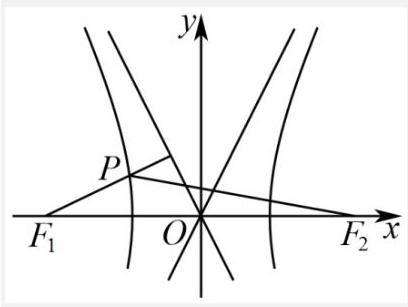
\includegraphics[width=0.2\textwidth]{bodyxb/src/bo_d2a13mv7aajc738pd0qg_0_245_868_408_307_0.jpg}
        \end{center}
        
        由 $\dfrac{\left| P{F}_{1}\right| }{\left| P{F}_{2}\right| } = \dfrac{2}{5}$ 得 $\left| {P{F}_{1}}\right|  = \dfrac{2}{5}\left| {P{F}_{2}}\right|$ ,又 $\left| {P{F}_{2}}\right|  - \left| {P{F}_{1}}\right|  = {2a}$ ,所以 $\left| {P{F}_{2}}\right|  = \dfrac{10a}{3},\left| {P{F}_{1}}\right|  = \dfrac{4a}{3}$
        
        $\cos \angle P{F}_{1}{F}_{2} = \dfrac{b}{c}$，由余弦定理得 ${\left| P{F}_{2}\right| }^{2} = {\left| P{F}_{1}\right| }^{2} + {\left| {F}_{1}{F}_{2}\right| }^{2} - 2\left| {P{F}_{1}}\right| \left| {{F}_{1}{F}_{2}}\right| \cos \angle P{F}_{1}{F}_{2}$ ,
        
        即 $\dfrac{{100}{a}^{2}}{9} = \dfrac{{16}{a}^{2}}{9} + 4{c}^{2} - \dfrac{16ab}{3}$ ,化简得 $3{\left( \dfrac{b}{a}\right) }^{2} - \dfrac{4b}{a} - 4 = 0$ ,即 $\left( {\dfrac{b}{a} - 2}\right) \left( {\dfrac{3b}{a} + 2}\right)  = 0$
        
        解得 $\dfrac{b}{a} = 2$ 或 $\dfrac{b}{a} =  - \dfrac{2}{3}$ ,因为 $a > 0,b > 0$ ,所以 $\dfrac{b}{a} = 2$ .
        
        则双曲线 $C$ 的渐近线方程为 $y =  \pm  {2x}$ .
    \end{jieda}

    \item 设 $M$ 是抛物线 ${y}^{2} = {4x}$ 上的一点, $F$ 是抛物线的焦点, $O$ 是坐标原点,若 $\angle {OFM} = {120}^{ \circ  }$ ,则 $\left| {FM}\right|$ 等于\blkda{4}
    \begin{jieda}
        过点 $M$ 作抛物线的准线 $l$ 的垂线,垂足为点 $N$ ,连接 ${FN}$，如图所示
        
        \begin{center}
        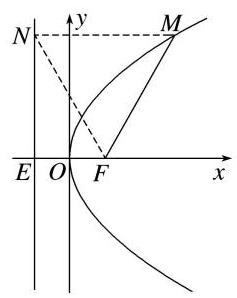
\includegraphics[width=0.2\textwidth]{bodyxb/src/bo_d1dpf7f7aajc73ecgk4g_7_707_1849_237_298_0.jpg}
        \end{center}

        因为 $\angle {OFM} = {120}^{ \circ  },{MN}//x$ 轴,则 $\angle {FMN} = {60}^{ \circ  }$ , 由抛物线的定义可得 $\left| {MN}\right|  = \left| {FM}\right|$ ,所以 $\bigtriangleup {FNM}$ 为等边三角形,则 $\angle {FNM} = {60}^{ \circ  }$ , 抛物线 ${y}^{2} = {4x}$ 的准线方程为 $x =  - 1$ ,设直线 $x =  - 1$ 交 $x$ 轴于点 $E$ 
        
        易知 $\left| {EF}\right|  = 2$ ,则 $\left| {FM}\right|  = \left| {FN}\right|  = 2\left| {EF}\right|  = 4$ . 
    \end{jieda}
\end{enumerate}
\subsection*{定义与数形结合}
\begin{enumerate}
    \item 若 $F$ 为椭圆 $C : \dfrac{{x}^{2}}{25} + \dfrac{{y}^{2}}{16} = 1$ 的右焦点, $A,B$ 为 $C$ 上两动点,则 $\bigtriangleup  {ABF}$ 周长的最大值为\blkda{20}
    \begin{jieda}
        如图,设 ${F}_{1}$ 为椭圆 $C$ 的左焦点,

        \begin{center}
        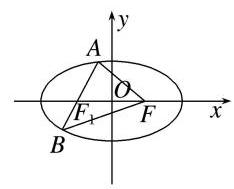
\includegraphics[width=0.2\linewidth]
        {bodyxb/src/01968c96-4637-7a01-8d97-98675cd6a1d6_4_704_314_234_189_0.jpg}
        \end{center}
        
        
        则由椭圆的定义可得 $\bigtriangleup {ABF}$ 的周长\\
        $\left| {AF}\right|  + \left| {BF}\right|  + \left| {AB}\right|  = {2a} - \left| {A{F}_{1}}\right|  + {2a} - \left| {B{F}_{1}}\right|  + \left| {AB}\right|  = {4a} + \left| {AB}\right|$  $- \left| {A{F}_{1}}\right|  - \left| {B{F}_{1}}\right|  = {20} + \left| {AB}\right|  - \left| {A{F}_{1}}\right|  - \left| {B{F}_{1}}\right|$\\
        当 $A,B,{F}_{1}$ 共线时, $\left| {AB}\right|  - \left| {A{F}_{1}}\right|  - \left| {B{F}_{1}}\right|  = 0$ , 当 $A,B,{F}_{1}$ 不共线时, $\left| {AB}\right|  - \left| {A{F}_{1}}\right|  - \left| {B{F}_{1}}\right|  < 0$ , 所以 $\bigtriangleup {ABF}$ 周长的最大值为 20 .
    \end{jieda}
    \item 已知双曲线的方程为 $\dfrac{{x}^{2}}{9} - \dfrac{{y}^{2}}{16} = 1$ ,点 ${F}_{1},{F}_{2}$ 是其左右焦点, ${A}$ 是圆 ${x}^{2} + {\left( y - 5\right) }^{2} = 4$ 上的一点,点 $M$ 在双曲线的右支上,则 $\left| {M{F}_{1}}\right|  + \left| {MA}\right|$ 的最小值是\blkda{$5\sqrt{2} + 4$}.
    \begin{jieda}
        由题意可得, ${c}^{2} = 9 + {16} = {25}$ ,即 $c = 5$ ,则 ${F}_{1},{F}_{2}$ 的坐标分别为 $\left( {-5,0}\right) ,\left( {5,0}\right)$，由双曲线的定义,得 $\left| {M{F}_{1}}\right|  - \left| {M{F}_{2}}\right|  = {2a} = 6$ 
        
        \begin{center}
        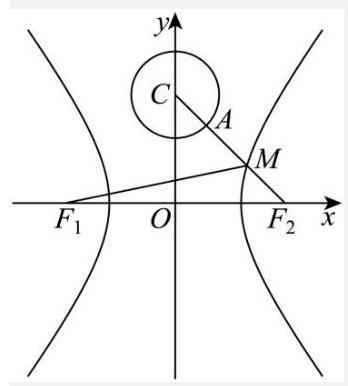
\includegraphics[width=0.2\textwidth]{bodyxb/src//bo_d3esa9s601uc738iqt8g_2_241_522_348_386_0.jpg}
        \end{center}

        又 ${A}$ 是圆 ${x}^{2} + {\left( y - 5\right) }^{2} = 4$ 上的点,设圆的圆心为 $C\left( {0,5}\right)$ ,半径为 $r = 2$
        
        由图可知, $\left| {CM}\right|  + \left| {M{F}_{2}}\right|  \geq  \left| {C{F}_{2}}\right|$，所以 $\left| {M{F}_{1}}\right|  + \left| {MA}\right|  = \left| {M{F}_{2}}\right|  + {2a} + \left| {MA}\right|  \geq  \left| {M{F}_{2}}\right|  + \left| {CM}\right|  + {2a} + {CA} \geq  C{F}_{2} + 6 - 2 = 5\sqrt{2} + 4$ ,
        
        当且仅当 $C$ 、 ${A}$ 、 $M$ 、 ${F}_{2}$ 四点共线( ${A}$ 、 $M$ 在 $C{F}_{2}$ 之间)时取等号,
        
        所以 $\left| {M{F}_{1}}\right|  + \left| {MA}\right|$ 的最小值为 $5\sqrt{2} + 4$
    \end{jieda}
    \item 已知点 $M\left( {{20},{40}}\right)$ 不在抛物线 $C : {y}^{2} = {2px}\left( {p > 0}\right)$ 上,抛物线 $C$ 的焦点为 $F$ . 若对于抛物线上的一点 $P,\left| {PM}\right|  + \left| {PF}\right|$ 的最小值为 41,则 $p$ 的值等于\blkda{42 或 22}.
    \begin{jieda}
        当$p = 40$时点$M$在抛物线上，当$0 < p < 40$的时候点$M$在抛物线外，当$p > 40$时点$M$在抛物线内.

        \twotu{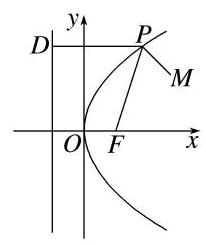
\includegraphics[width=0.2\textwidth]{bodyxb/src/bo_d1dpf7f7aajc73ecgk4g_2_583_795_206_245_0.jpg}}{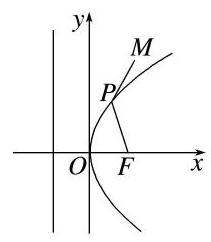
\includegraphics[width=0.2\textwidth]{bodyxb/src/bo_d1dpf7f7aajc73ecgk4g_2_853_796_211_242_0.jpg}}
        
        \begin{dingautolist}{172}
            \item 如左图所示，当点 $M\left( {{20},{40}}\right)$ 位于抛物线内时，过点 $P$ 作抛物线准线的垂线，垂足为 $D$，则 $\left| {PF}\right|  = \left| {PD}\right|$，因此有$\left| {PM}\right|  + \left| {PF}\right|  = \left| {PM}\right|  + \left| {PD}\right| .$

            当点 $M,P,D$ 三点共线时，$\left| {PM}\right|  + \left| {PF}\right|$ 的值最小.
            
            由最小值为 41，得 ${20} + \dfrac{p}{2} = {41}$ ,解得 $p = {42}$，符合要求.
            \item 如右图所示，当点 $M\left( {{20},{40}}\right)$ 位于抛物线上及抛物线外时，当点 $P,M,F$ 三点共线时, $\left| {PM}\right|  + \left| {PF}\right|$ 的值最小.

            由最小值为 41，得 $\sqrt{{40}^{2} + {\left( {20} - \dfrac{p}{2}\right) }^{2}} = {41}$，解得 $p = {22}$ 或 $p = {58}$（舍）.
        \end{dingautolist}
        综上, $p = {42}$ 或 $p = {22}$ .
    \end{jieda}
\end{enumerate}

\subsection*{标准方程}
\begin{enumerate}
    \item “ $1 < k < 5$ ” 是方程 “ $\dfrac{{x}^{2}}{k - 1} + \dfrac{{y}^{2}}{5 - k} = 1$ 表示椭圆” 的\dotfill{(\kh{A})}
    \xx{必要不充分条件}{充分不必要条件}{充要条件}{既不充分也不必要条件}
    \item 当实数 $k$ 为何值时,方程 $\dfrac{{x}^{2}}{{25} - k} + \dfrac{{y}^{2}}{9 - k} = 1$ 表示的曲线是椭圆或双曲线? 并指出它们的共同特征.
    \begin{jieda}
        只要满足$25-k>0$或$9-k>0$，即$k \in (-\infty, 9)$方程所表示的曲线就是椭圆或者双曲线
        
        因为$25-k > 9-k$，因此无论方程表示椭圆还是双曲线，都是有$a^2 = 25-k, b^2 = |9-k|$，因此$c = 4$，即焦点为$(4, 0)$和$(-4, 0)$
    \end{jieda}
    \item 求满足下列条件的椭圆的标准方程：焦距是6,且过点(0,4)
    \begin{jieda}
        根据条件可知$c = 3$
            \begin{dingautolist}{172}
                \item 若焦点在$x$轴上，则$b = 4$，$a^2 = 16+9 = 25$，故标准方程为$\dfrac{x^2}{25} + \dfrac{y^2}{16} = 1$
                \item 若焦点在$y$轴上，则$a = 4$，$b^2 = 16-9 = 7$，故标准方程为$\dfrac{x^2}{7} + \dfrac{y^2}{16} = 1$
            \end{dingautolist}
    \end{jieda}
    \item 求满足下列条件的双曲线的标准方程:
    \begin{dingautolist}{172}
        \item 一条渐近线为 ${2x} - {3y} = 0$ ,且过点$(1, -1)$
        \item 焦点在$x$轴上，过点 $\left( {\sqrt{2},\sqrt{3}}\right)$ ,且离心率为 2
    \end{dingautolist}
    \begin{jieda}
        \begin{dingautolist}{172}
            \item 设双曲线方程为$\dfrac{x^2}{9} - \dfrac{y^2}{4} = k$，代入$(1, -1)$，故$k = -\dfrac{5}{36}$，因此双曲线的标准方程为$\dfrac{y^2}{\dfrac{5}{9}}-\dfrac{x^2}{\dfrac{5}{4}} = 1$
            \item 由 $e = \dfrac{c}{a} = 2$，得 $c = {2a}, b = \sqrt{{c}^{2} - {a}^{2}} = \sqrt{3}a$，则双曲线的方程为 $x^2 - \dfrac{{y}^{2}}{3} = {a}^{2}$ 
            
            将点 $\left( {\sqrt{2},\sqrt{3}}\right)$ 的坐标代入双曲线的方程可得 $a = 1$ ,故双曲线的标准方程为 ${x}^{2} - \dfrac{{y}^{2}}{3} = 1$.
        \end{dingautolist}
    \end{jieda}
    \item 若抛物线 $y = a{x}^{2}$ 的焦点到准线的距离为 2 ,则实数 $a =$\blkda{$\pm \dfrac{1}{4}$}
    \begin{jieda}
        ${x}^{2} = \dfrac{1}{a}y$，故$\dfrac{1}{2|a|} = 2$，即$a = \pm \dfrac{1}{4}$
    \end{jieda}
\end{enumerate}
\subsection*{圆锥曲线的统一定义}
\begin{enumerate}
    \item 如图，椭圆 \ding{172} ， \ding{173} 与双曲线 \ding{174} ， \ding{175}的离心率分别为 $e_1,e_2,e_3,e_4$ ，其大小关系为\blkda{$e_1 < e_2 < e_4 < e_3$}.
    \begin{center}
    \includegraphics[width=0.2\textwidth]{bodyxb/src/0_147_394_524_340_0.jpg}
    \end{center}
    \item 已知椭圆 $\dfrac{x^2}{4} + \dfrac{y^2}{3} = 1$ 内有一点 $P(1, - 1) ,F$ 是椭圆的右焦点，点 $M$ 在椭圆上，则 $|MP| + 2|MF|$ 的最小值是\blkda{3}，此时点 $M$ 的坐标为\blkda{$\left( \frac{2\sqrt{6}}{3}, - 1\right)$}.
    \begin{jieda}
        由椭圆的方程,可知 $a = 2,b = \sqrt{3},c = 1$ ,所以 $e = \frac{1}{2}$ ,右准线 $l : x = \frac{a^2}{c} = 4$ .

        如图,设 $M$ 在右准线 $l : x = 4$ 上的射影为 $M_1$ ,

        根据椭圆的第二定义,有 $e = \frac{|MF|}{|MM_1|} = \frac{1}{2}$ ,即 $2|MF| = |MM_1|$ ,所以 $|MP| + 2|MF| = |MP| + |MM_1|$ .

        显然,当 $P\text{ 、 }M\text{ 、 }M_1$ 三点共线时, $|MP| + |MM_1|$ 有最小值,

        即 $\left( |MP| + 2|MF|\right)_{\min} = \frac{a^2}{c} - x_P = 4 - 1 = 3$ .

        此时 $y_M = y_P = - 1$ ,将 $y_M = - 1$ 代入椭圆的方程得 $x_M = \frac{2\sqrt{6}}{3}$ 或 $x_M = - \frac{2\sqrt{6}}{3}$ (舍去),所以 $M\left( \frac{2\sqrt{6}}{3}, - 1\right)$ .

        \begin{center}
        \includegraphics[width=0.3\textwidth]{bodyxb/src/2_145_1093_391_288_0.jpg}
        \end{center}
    \end{jieda}
\end{enumerate}
\subsection*{焦点三角形与等面积法}
\begin{enumerate}
    \item 已知 ${F}_{1},{F}_{2}$ 为椭圆 $\dfrac{{x}^{2}}{{a}^{2}} + \dfrac{{y}^{2}}{{b}^{2}} = 1\left( {a > b > 0}\right)$ 的左、右焦点,椭圆的离心率为 $\dfrac{1}{2},M$ 为椭圆上一动点,则 $\angle {F}_{1}M{F}_{2}$ 的最大值为\blkda{$\dfrac{\pi}{3}$}
    \begin{jieda}
        设$\theta = \angle {F}_{1}M{F}_{2}$，
        $S_{\triangle {F}_{1}M{F}_{2}} = b^2tan\dfrac{\theta}{2}$，易知当$M$位于短轴顶点上的时候焦点三角形面积最大，即$tan\dfrac{\theta}{2}$，即$\theta$最大. \\
        此时根据几何关系有$sin\dfrac{\theta}{2} = e = \dfrac{1}{2}$，故$\dfrac{\theta}{2} = \dfrac{\pi}{6}$，所以$\theta = \dfrac{\pi}{3}$
    \end{jieda}
    \item 已知椭圆 $\dfrac{{x}^{2}}{9} + \dfrac{{y}^{2}}{4} = 1$ 的焦点为 ${F}_{1}$ 、 ${F}_{2}$ ,点 $P$ 为椭圆上的动点,当 $\angle {F}_{1}P{F}_{2}$ 是钝角时,则 $P$ 的横坐标的范围是\blkda[4]{$\left(-\dfrac{3\sqrt{5}}{5},\dfrac{3\sqrt{5}}{5}\right)$}.
    \item 如图, ${F}_{1}$ 、 ${F}_{2}$ 是椭圆 ${C}_{1} : \dfrac{{x}^{2}}{{a}^{2}} + \dfrac{{y}^{2}}{{b}^{2}} = 1$ 与双曲线 ${C}_{2} : \dfrac{{x}^{2}}{5} - {y}^{2} = 1$ 的公共焦点, $A$ 、 $B$ 分别是 ${C}_{1}$ 、${C}_{2}$ 在第二、四象限的公共点,若四边形 $A{F}_{1}B{F}_{2}$ 为矩形,则 ${C}_{1}$ 的离心率是\blkda{$\dfrac{\sqrt{42}}{7}$}.
    \begin{center}
        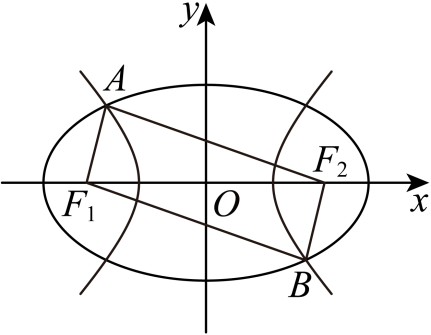
\includegraphics[width=0.2\linewidth]{bodyxb//src/jiaodiansanjiaoxing1.png}
    \end{center}
\end{enumerate}
\subsection*{焦点三角形多解}
\begin{enumerate}
    \item 已知点 $P$ 是椭圆 $\dfrac{y^2}{45} + \dfrac{x^2}{9} = 1$ 上一点，点 $F_1$ 、 $F_2$ 是椭圆上、下焦点， $\Delta F_{1}PF_2$ 有一个内角为 $\dfrac{2\pi}{3}$ ，则 $\Delta F_{1}PF_2$ 的面积为\blkda[4]{$9\sqrt{3}$ 或 $\dfrac{9}{4}\left( \sqrt{15} - \sqrt{3}\right)$}
        
    \item 在 $\bigtriangleup ABC$ 中, $AB = 3,AC = 5,BC = \sqrt{14}$ . 已知点 $A,B,C$ 分别为椭圆的上、下、右顶点,以及两个焦点中的三点,求椭圆的离心率\blkda{$\dfrac{2}{3}$}
\end{enumerate}
\subsection*{焦点三角形中位线}
\begin{enumerate}
    \item 已知椭圆 $\dfrac{{x}^{2}}{9} + \dfrac{{y}^{2}}{5} = 1$ 的左、右焦点分别为 ${F}_{1},{F}_{2}$ ,点 $P$ 在椭圆上,设线段 $P{F}_{1}$ 的中点为 $M$ ,且 $\left| {O{F}_{2}}\right|  = \left| {OM}\right|$ ,则 $\bigtriangleup  P{F}_{1}{F}_{2}$ 的面积为\blkda{$\sqrt{15}$}
    \begin{jieda}
        根据标准方程可知$a = 3, c = \sqrt{9-5} = 2$，根据几何关系可知$PF_2 = 2c = 4, PF_1 = 2$，故$\triangle{PF_1F_2}$为等腰三角形. \\
        根据余弦定理可得$cos\angle PF_2F_1 = \dfrac{16+16-4}{2\times 4\times 4} = \dfrac{7}{8}$，故$sin\angle PF_2F_1 = \dfrac{\sqrt{15}}{8}$，故$S = \dfrac{1}{2} \times 4 \times 4 \times \dfrac{\sqrt{15}}{8} = \sqrt{15}$
    \end{jieda}
    \item 已知双曲线 $\dfrac{{x}^{2}}{4} - \dfrac{{y}^{2}}{5} = 1$ 的左焦点为 $F$ ,点 $P$ 在双曲线上且在 $x$ 轴上方,若线段 ${PF}$ 的中点在以 $O$ 为圆心, $\left| {OF}\right|$ 为半径的圆上,则直线 ${PF}$ 的斜率为\blkda[3]{$\dfrac{\sqrt{11}}{5}$ 或 $\sqrt{35}$}.
    \begin{jieda}
        由双曲线 $\dfrac{{x}^{2}}{4} - \dfrac{{y}^{2}}{5} = 1$ 可知 $a = 2,b = \sqrt{5},c = \sqrt{{a}^{2} + {b}^{2}} = 3$ ,
        
        设线段 ${PF}$ 的中点为 $M$ ,双曲线的右焦点为 ${A}$，则 $\left| {OM}\right|  = 3,\left| {AF}\right|  = 6$
        \begin{center}
            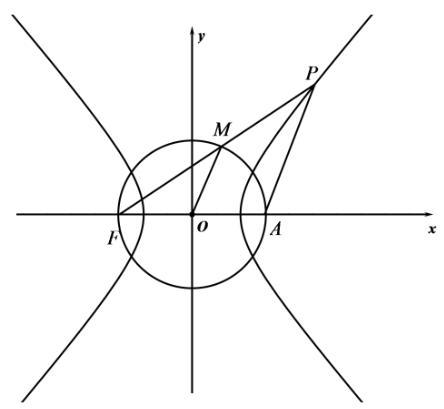
\includegraphics[width=0.2\textwidth]{bodyxb/src/bo_d3eri7s601uc738iqr70_2_240_1616_444_409_0.jpg}
        \end{center}
        \begin{dingautolist}{172}
            \item 若点 $P$ 在第一象限,则 $\left| {PA}\right|  = 2\left| {OM}\right|  = 6,\left| {PF}\right|  = \left| {PA}\right|  + 4 = {10}$，可得 $\cos \angle {PFA} = \dfrac{{\left| PA\right| }^{2} + {\left| AF\right| }^{2} - {\left| AP\right| }^{2}}{2\left| {PA}\right|  \cdot  \left| {AF}\right| } = \dfrac{{10}^{2} + {6}^{2} - {6}^{2}}{2 \times  {10} \times  6} = \dfrac{5}{6}$，则 $\sin \angle {PFA} = \sqrt{1 - {\cos }^{2}\angle {PFA}} = \dfrac{\sqrt{11}}{6}$
            
            可得 $\tan \angle {PFA} = \dfrac{\sin \angle {PFA}}{\cos \angle {PFA}} = \dfrac{\sqrt{11}}{5}$ ,所以直线 ${PF}$ 的斜率为 $\dfrac{\sqrt{11}}{5}$ .
            
            \item 若点 $P$ 在第二象限，则$\left| {PA}\right|  = 2\left| {OM}\right|  = 6,\left| {PF}\right|  = \left| {PA}\right|  - 4 = 2$

            ，可得 $\cos \angle {PFA} = \dfrac{{\left| PA\right| }^{2} + {\left| AF\right| }^{2} - {\left| AP\right| }^{2}}{2\left| {PA}\right|  \cdot  \left| {AF}\right| } = \dfrac{2^{2} + {6}^{2} - {6}^{2}}{2 \times  2 \times  6} = \dfrac{1}{6}$，$\sin \angle {PFA} = \sqrt{1 - {\cos }^{2}\angle {PFA}} = \dfrac{\sqrt{35}}{6}$

            可得 $\tan \angle {PFA} = \dfrac{\sin \angle {PFA}}{\cos \angle {PFA}} = \sqrt{35}$ ,所以直线 ${PF}$ 的斜率为 $\sqrt{35}$ .
        
        \end{dingautolist}
        \ps 直接求解$\left\{  \begin{array}{l} \dfrac{{\left( s - 3\right) }^{2}}{4} + \dfrac{81}{4} = 9 \\  \dfrac{{s}^{2}}{4} - \dfrac{81}{5} = 1  \\  t > 0 \end{array}\right.$即可得$P$在一二两个象限的坐标$(s, t)$.
    \end{jieda}
    \item 如图,已知 $F$ 是椭圆 $\dfrac{{x}^{2}}{4} + \dfrac{{y}^{2}}{3} = 1$ 的左焦点, $A$ 为椭圆的下顶点,点 $P$ 是椭圆上任意一点,以 ${PF}$ 为直径作圆 $N$ ,射线 ${ON}$ 与圆 $N$ 交于点 $Q$ ,则 $\left| {AQ}\right|$ 的取值范围为\blkda[3]{$\left\lbrack  {2 - \sqrt{3},2 + \sqrt{3}}\right\rbrack$}.
    
    \begin{center}
    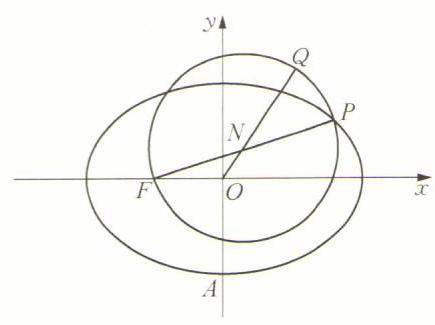
\includegraphics[width=0.2\textwidth]{bodyxb/src/bo_d1ig044601uc738hj6v0_93_1055_1304_435_325_0.jpg}
    \end{center}
    \begin{jieda}
        设 ${F}_{1}$ 为椭圆的右焦点，因为 $O$ , $N$ 分别为 $F{F}_{1}$, ${PF}$ 的中点，所以 $\left| {ON}\right|  = \dfrac{1}{2}\left| {P{F}_{1}}\right|$，$\left|{NQ}\right|  =  \dfrac{1}{2}\left| {PF}\right|$，因此$\left| {OQ}\right|  = \left| {ON}\right|  + \left| {NQ}\right|  = \dfrac{1}{2}\left( {\left| {PF}\right|  + \left| {P{F}_{1}}\right| }\right)  = 2$
        
        所以 $Q$ 的轨迹是以 $O$ 为圆心,以2为半径的圆, $A(0, - \sqrt{3})$ 在圆内，所以数形结合可知$\left| {AQ}\right|$ 的取值范围为 $\left\lbrack  {2 - \sqrt{3},2 + \sqrt{3}}\right\rbrack$ .
    \end{jieda}
    \item 已知 ${F}_{1}$ 、 ${F}_{2}$ 是椭圆 $\dfrac{{x}^{2}}{4} + \dfrac{{y}^{2}}{3} = 1$ 的左、右焦点,点 $P$ 是椭圆上任意一点,以 $P{F}_{1}$ 为直径作圆 $N$ ,直线 ${ON}$ 与圆 $N$ 交于点 $Q$ (点 $Q$ 不在椭圆内部),则 $\vv{Q{F}_{1}} \cdot  \vv{Q{F}_{2}} =$ \blkda{3}
    \begin{jieda}
        连接 $P{F}_{2}$ ,设椭圆的基本量为 $a,b,c$ ,
        \begin{center}
        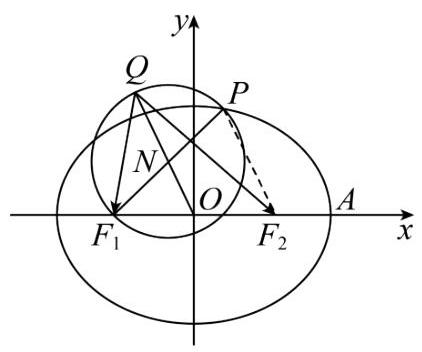
\includegraphics[width=0.2\textwidth]{bodyxb/src/bo_d37kc177aajc738v9fhg_2_240_962_422_352_0.jpg}
        \end{center}
        $\vv{Q{F}_{1}} \cdot  \vv{Q{F}_{2}} = \left( {\vv{QO} + \vv{O{F}_{1}}}\right)  \cdot  \left( {\vv{QO} + \vv{O{F}_{2}}}\right)  = {\left( \vv{QO}\right) }^{2} - {\left( \vv{O{F}_{1}}\right) }^{2},$
        
        $= {\left( \left| QN\right|  + \left| NO\right| \right) }^{2} - {c}^{2} = {\left( \dfrac{\left| P{F}_{1}\right| }{2} + \dfrac{\left| P{F}_{2}\right| }{2}\right) }^{2} - {c}^{2} = {a}^{2} - {c}^{2} = {b}^{2} = 3$
    \end{jieda}
    \item 已知双曲线 $E : \dfrac{{x}^{2}}{{a}^{2}} - \dfrac{{y}^{2}}{{b}^{2}} = 1\left( {a > 0,b > 0}\right)$ 的左、右焦点分别为 ${F}_{1}\text{、}{F}_{2}$ ,过点 ${F}_{1}$ 的直线 $l$ 交 $E$ 的左支于 $A,B$ 两点. 若 $\left| {OB}\right|  = \left| {O{F}_{1}}\right|$ ( $O$ 为坐标原点),且点 $O$ 到直线 $l$ 的距离为 $\dfrac{3}{2}a$ ,则该双曲线的两条渐近线的夹角为\blkda[3]{$arctan\left(2\sqrt{6}\right)$}.
        \begin{jieda}
            令双曲线 $E$ 的半焦距为 $c$ ,取 ${F}_{1}B$ 的中点 $D$ ,连接 ${OD}$ ,由 $\left| {OB}\right|  = \left| {O{F}_{1}}\right|$，得 ${OD}\bot {F}_{1}B$ , $\left| {OD}\right|  = \dfrac{3}{2}a$ ,连接 ${F}_{2}B$ ,由 $O$ 为 ${F}_{1}{F}_{2}$ 的中点,得 $B{F}_{2}//{OD}$，则 $\left| {B{F}_{2}}\right|  = 2\left| {OD}\right|  = {3a}$ , $B{F}_{2} \bot  B{F}_{1}$ , $\left| {{F}_{1}B}\right|  = \left| {B{F}_{2}}\right|  - {2a} = a$
            \begin{center}
                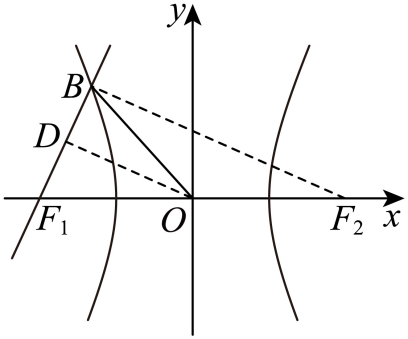
\includegraphics[width=0.2\linewidth]{bodyxb//src/shuangquxianzhongweixian1.png}
            \end{center}
            因此 ${\left| B{F}_{2}\right| }^{2} + {\left| B{F}_{1}\right| }^{2} = {\left| {F}_{1}{F}_{2}\right| }^{2}$ ,即 ${\left( 3a\right) }^{2} + {a}^{2} = {\left( 2c\right) }^{2}$ ,整理得 $5{a}^{2} = 2{c}^{2}$

            故$e^2 = \dfrac{5}{2}$，即渐近线斜率$k$满足$k^2 = e^2-1 = \dfrac{3}{2}$，因此$k = \pm \dfrac{\sqrt{6}}{2}$

            \begin{dingautolist}{172}
                \item $\theta = \pi - 2arctan\left(\dfrac{\sqrt{6}}{2}\right)$
                \item $tan\theta = \left|\dfrac{2 \times \dfrac{\sqrt{6}}{2}}{1-\left(\dfrac{\sqrt{6}}{2}\right)^2}\right| = 2\sqrt{6}$，故$\theta = arctan\left(2\sqrt{6}\right)$
            \end{dingautolist}
        \end{jieda}

    \item 已知 ${F}_{1}$ , ${F}_{2}$ 分别为双曲线 $C : \dfrac{{x}^{2}}{{a}^{2}} - \dfrac{{y}^{2}}{{b}^{2}} = 1\left( {a > 0,b > 0}\right)$ 的左,右焦点, $O$ 为坐标原点,以点 ${F}_{2}$ 为圆心且与 $C$ 的渐近线相切的圆与 $C$ 在第一象限交于点 $A,B$ 为 $A{F}_{1}$ 的中点,若 $\vv{OB} \cdot  \vv{B{F}_{2}} = 0$ ,则 $C$ 的渐近线的斜率为\blkda{$\pm  \dfrac{2}{3}$}
        
    \begin{jieda}
        设双曲线 $\dfrac{{x}^{2}}{{a}^{2}} - \dfrac{{y}^{2}}{{b}^{2}} = 1$ 的半焦距为 $c$，由题意 ${F}_{2}\left( {c,0}\right)$ ,双曲线的一条渐近线为 $y = \dfrac{b}{a}x$ ,
        则点 ${F}_{2}$ 到渐近线 ${bx} - {ay} = 0$ 的距离 $d = \dfrac{\left| bc\right| }{\sqrt{{b}^{2} + {\left( -a\right) }^{2}}} = b$，即圆 ${F}_{2}$ 的半径为 $b$ 
        
        \begin{center}
        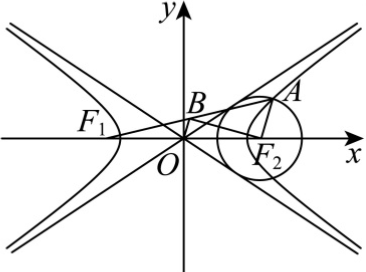
\includegraphics[width=0.2\linewidth]{bodyxb//src/jianjinxian1.png}
        \end{center}
        连接 $A{F}_{2}$ ,则 $\left| {A{F}_{2}}\right|  = b$，由双曲线的定义知 $\left| {A{F}_{1}}\right|  - \left| {A{F}_{2}}\right|  = {2a}$ ,
        所以 $\left| {B{F}_{1}}\right|  = \dfrac{1}{2}\left| {A{F}_{1}}\right|  = \dfrac{1}{2}\left( {{2a} + \left| {A{F}_{2}}\right| }\right)  = a + \dfrac{b}{2}$ .
        
        在 ${\triangle A}{F}_{1}{F}_{2}$ 中, $O$ 为 ${F}_{1}{F}_{2}$ 的中点, $B$ 为 $A{F}_{1}$ 的中点,
        所以 $\left| {OB}\right|  = \dfrac{1}{2}\left| {A{F}_{2}}\right|  = \dfrac{b}{2}$

        在Rt $\bigtriangleup {OB}{F}_{2}$ 中, $\cos \angle {BO}{F}_{2} = \dfrac{\left| OB\right| }{\left| O{F}_{2}\right| } = \dfrac{b}{2c}$
        
        在 ${\triangle OB}{F}_{1}$ 中, $\cos \angle {BO}{F}_{1} = \dfrac{{\left| OB\right| }^{2} + {\left| O{F}_{1}\right| }^{2} - {\left| B{F}_{1}\right| }^{2}}{2\left| {OB}\right|  \cdot  \left| {O{F}_{1}}\right| } = \dfrac{\dfrac{{b}^{2}}{4} + {c}^{2} - {\left( a + \dfrac{b}{2}\right) }^{2}}{2 \cdot  \dfrac{b}{2} \cdot  c} = \dfrac{{c}^{2} - {a}^{2} - {ab}}{bc} = \dfrac{b - a}{c}$ .
        
        因为 $\cos \angle {BO}{F}_{1} =  - \cos \angle {BO}{F}_{2}$ ,所以 $\dfrac{b - a}{c} =  - \dfrac{b}{2c}$ ,所以 $\dfrac{b}{a} = \dfrac{2}{3}$ ,
        所以双曲线的渐近线的斜率为 $\pm  \dfrac{2}{3}$
    \end{jieda}
\end{enumerate}
\subsection*{导比例解三角求离心率}
\begin{enumerate}
    \item 古希腊数学家阿波罗尼奥斯在研究圆锥曲线时发现了椭圆的光学性质:从椭圆的一个焦点射出的光线, 经椭圆反射, 其反射光线必经过椭圆的另一焦点. 设椭圆方程 $\dfrac{{x}^{2}}{{a}^{2}} + \dfrac{{y}^{2}}{{b}^{2}} = 1\left( {a > b > 0}\right) ,{F}_{1}$ 、 ${F}_{2}$ 为其左、右焦点,若从右焦点 ${F}_{2}$ 发出的光线经椭圆上的点 ${A}$ 和点 $B$ 反射后,满足 ${AB} \bot  {AD},\cos \angle {ABC} = \dfrac{4}{5}$ ,则该椭圆的离心率为\blkda{$\dfrac{\sqrt{2}}{2}$}.
    \begin{center}
    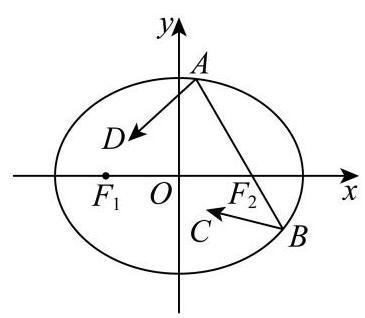
\includegraphics[width=0.2\textwidth]{bodyxb/src/bo_d43fvmc601uc738mn8og_3_214_355_365_318_0.jpg}
    \end{center}
    
    \begin{jieda}
        由题意, 可作图如下:
        
        \begin{center}
        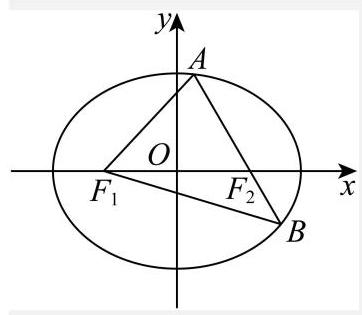
\includegraphics[width=0.2\textwidth]{bodyxb/src/bo_d43g3ak601uc738mn9ng_0_241_1253_362_315_0.jpg}
        \end{center}
        
        则 $\cos \angle {AB}{F}_{1} = \dfrac{4}{5} = \dfrac{\left| AB\right| }{\left| B{F}_{1}\right| },\sin \angle {AB}{F}_{1} = \sqrt{1 - {\cos }^{2}\angle {AB}{F}_{1}} = \dfrac{3}{5} = \dfrac{\left| A{F}_{1}\right| }{\left| B{F}_{1}\right| }$ ,即 $\left| {AB}\right|  : \left| {A{F}_{1}}\right|  : \left| {B{F}_{1}}\right|  = 4 : 3 : 5$ , 可设 $\left| {AB}\right|  = {4k}$ , $\left| {A{F}_{1}}\right|  = {3k}$ , $\left| {B{F}_{1}}\right|  = {5k}$ ,
        
        由 $\left| {AB}\right|  + {\left| AF\right| }_{1} + \left| {B{F}_{1}}\right|  = \left| {A{F}_{2}}\right|  + \left| {B{F}_{2}}\right|  + \left| {A{F}_{1}}\right|  + \left| {B{F}_{1}}\right|  = {4a}$ ,则 ${4k} + {3k} + {5k} = {4a}$ ,即 ${3k} = a$ ,
        
        $\left| {A{F}_{2}}\right|  = {2a} - \left| {A{F}_{1}}\right|  = {3k}$ ,在 Rt $\bigtriangleup A{F}_{1}{F}_{2}$ 中, $\left| {{F}_{1}{F}_{2}}\right|  = \sqrt{{\left| A{F}_{1}\right| }^{2} + {\left| A{F}_{2}\right| }^{2}} = 3\sqrt{2}k = {2c}$ ,
        
        则 $e = \dfrac{2c}{2a} = \dfrac{3\sqrt{2}k}{6k} = \dfrac{\sqrt{2}}{2}$ .
    \end{jieda}
    \item 已知双曲线 $C : \dfrac{{x}^{2}}{{a}^{2}} - \dfrac{{y}^{2}}{{b}^{2}} = 1\left( {a > 0,b > 0}\right)$ 的左、右焦点分别为 ${F}_{1},{F}_{2}$ . 点 ${A}$ 在 $C$ 上,点 $B$ 在 $y$ 轴上, $\vv{{F}_{1}A} \bot  \vv{{F}_{1}B},\vv{{F}_{2}A} =  - \dfrac{2}{3}\vv{{F}_{2}B}$ ,则 $C$ 的离心率为\blkda{$\dfrac{3\sqrt{5}}{5}$}
    \begin{jieda}
        示意图如下
        \begin{center}
        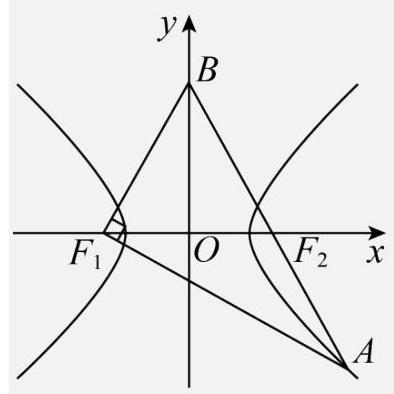
\includegraphics[width=0.2\textwidth]{bodyxb/src/bo_d2a0hlbef24c73avno0g_1_237_1565_394_394_0.jpg}
        \end{center}
        设$|F_2B| = 3m$，则$|F_2A| = 2m$，故$|F_1B| = 3m, |F_1A| = 2a+2m$，根据勾股定理可得$m = a$，因此$cos\angle{ABF_1} = \dfrac{3}{5}$，故在$\triangle F_1BF_2$中根据余弦定理有$\dfrac{3}{5} = \dfrac{9a^2+9a^2-4c^2}{2\times 3a \times 3a} = \dfrac{18a^2-4c^2}{18a^2}$，故$e = \dfrac{3\sqrt{5}}{5}$
    \end{jieda}
\end{enumerate}
\subsection*{椭圆的焦半径公式}
\begin{enumerate}
    \item 如图,把椭圆 $\dfrac{{x}^{2}}{25} + \dfrac{{y}^{2}}{16} = 1$ 的长轴 ${AB}$ 分成 8 等份,过每个分点作 $x$ 轴的垂线交椭圆的上半部分于 ${P}_{1},{P}_{2},{P}_{3},{P}_{4},{P}_{5},{P}_{6},{P}_{7}$ 七个点, $F$ 是椭圆的一个焦点,则$\left| {{P}_{1}F}\right|  + \left| {{P}_{2}F}\right|  + \left| {{P}_{3}F}\right|  + \left| {{P}_{4}F}\right|  + \left| {{P}_{5}F}\right|  + \left| {{P}_{6}F}\right|  + \left| {{P}_{7}F}\right|  =$ \blkda{35}
    \begin{center}
        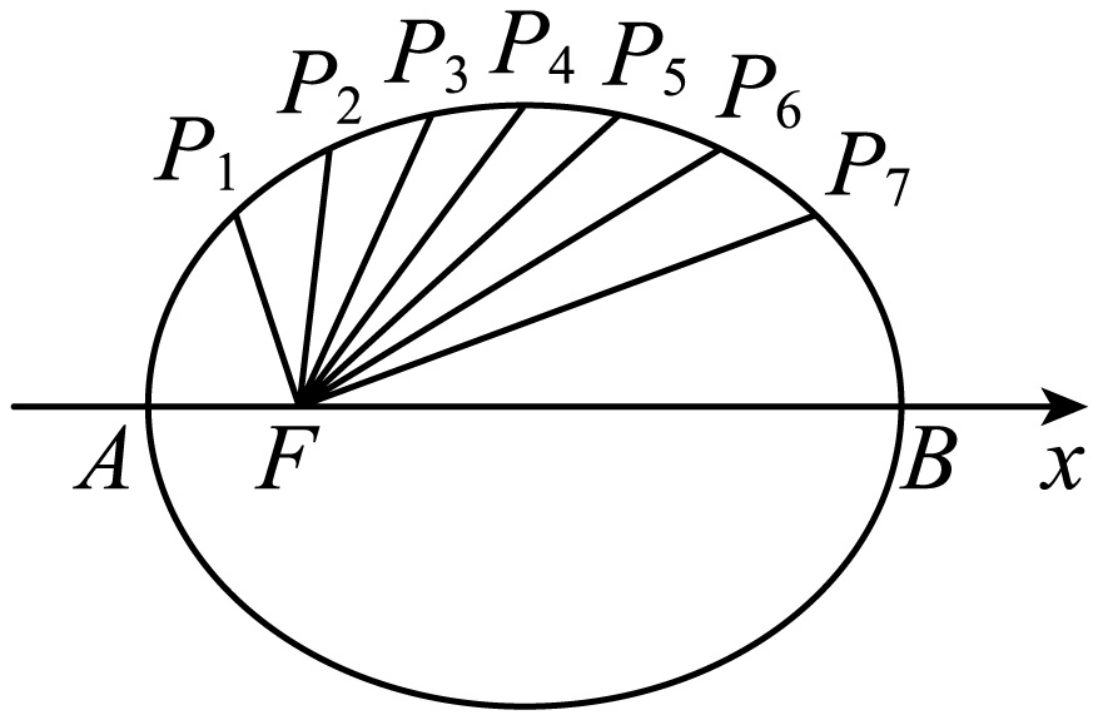
\includegraphics[width=0.2\linewidth]{bodyxb//src/jiaobanjing.png}
    \end{center}
        
    \begin{jieda}
        $\left| {{P}_{1}F}\right|  + \left| {{P}_{2}F}\right|  + \left| {{P}_{3}F}\right|  + \left| {{P}_{4}F}\right|  + \left| {{P}_{5}F}\right|  + \left| {{P}_{6}F}\right|  + \left| {{P}_{7}F}\right|  = 7a + e(x_1+x_2 +...+x_7) = 7a = 35$
    \end{jieda}
    
    \item 已知 $\bigtriangleup {ABC}$ 是椭圆 $\dfrac{{y}^{2}}{9} + \dfrac{{x}^{2}}{{b}^{2}} = 1\left( {3 > b > 0}\right)$ 的内接三角形, $F$ 是椭圆的上焦点,且原点 $O$是 $\bigtriangleup  {ABC}$ 的重心. 求 $A,B,C$ 三点到 $F$ 距离之和为\blkda{9}
    \begin{jieda}
        原式$= 3a - e(y_1+y_2+y_3) = 3a = 9$.
    \end{jieda}

    \item 已知 $F_1,F_2$ 是椭圆 $C : \dfrac{x^2}{9} + \dfrac{y^2}{4} = 1$ 的两个焦点，点 $M$ 在 $C$ 上，则 $\dfrac{1}{|MF_1|} + \dfrac{1}{|MF_2|}$ 的最小值为\blkda{$\dfrac{2}{3}$}
    \begin{jieda}
        $\dfrac{1}{a+ex_0}+\dfrac{1}{a-ex_0} = \dfrac{2a}{a^2-e^2x_0^2} \geq \dfrac{2}{a} = \dfrac{2}{3}$
    \end{jieda}
\end{enumerate}
\subsection*{抛物线的焦半径公式}
\begin{enumerate}
    \item 过抛物线 ${y}^{2} = {4x}$ 的焦点的直线 $l$ 交抛物线于 $P\left( {{x}_{1},{y}_{1}}\right) ,Q\left( {{x}_{2},{y}_{2}}\right)$ 两点,如果 ${x}_{1} + {x}_{2} = 6$ ,则 $\left| {PQ}\right|$ 等于\blkda{8}
    \begin{jieda}
        抛物线 ${y}^{2} = {4x}$ 的焦点为 $F\left( {1,0}\right)$ ,准线方程为 $x =  - 1$. 根据题意可得，$\left| {PQ}\right|  = \left| {PF}\right|  + \left| {QF}\right|  = {x}_{1} + 1 + {x}_{2} + 1 = {x}_{1} + {x}_{2} + 2 = 8$ .
    \end{jieda}
    \item 在抛物线 ${y}^{2} = {8x}$ 上有$A,B,C$三点，$F$ 为其焦点,且 $F$ 为 $\bigtriangleup  {ABC}$ 的重心,则 $\left| {AF}\right|  + \left| {BF}\right|  + \left| {CF}\right|$ 等于\blkda{12}
    \begin{jieda}
        ${y}^{2} = {8x}$的焦点为$(2, 0)$，准线为$x = -2$
        
        根据抛物线的定义可知$|AF|$等于$A$到准线的距离，即$|AF| = x_A + 2$，同理可有$|BF| = x_B + 2, |CF| = x_C + 2$
    
        因为$F$ 为 $\bigtriangleup  {ABC}$ 的重心，所以$3x_F = x_A + x_B + x_C$，故$\left| {AF}\right|  + \left| {BF}\right|  + \left| {CF}\right| = x_A + x_B + x_C + 6 = 3x_F + 6 = 12$
    \end{jieda}
\end{enumerate}
\subsection*{带倾斜角的焦半径公式}
\begin{center}
    \begin{tabular}{|c|c|c|c|c|}
    \hline
    {$\alpha$为锐角、焦点在$x$轴上} & 椭圆 & 双曲线（交一支） &  双曲线（交两支）& 抛物线 \\
    \cline{1-5}
    长焦半径 & $\dfrac{ep}{1-ecos\alpha}$ & $\dfrac{ep}{1-ecos\alpha}$ & $-\dfrac{ep}{1-ecos\alpha}$ & $\dfrac{p}{1-cos\alpha}$ \\    
    \cline{1-5}
    短焦半径 & $\dfrac{ep}{1+ecos\alpha}$ & $\dfrac{ep}{1+ecos\alpha}$ & $\dfrac{ep}{1+ecos\alpha}$ & $\dfrac{p}{1+cos\alpha}$ \\
    \cline{1-5}
    焦点弦长 & $\dfrac{2ep}{1-e^2cos^2\alpha}$ & $\dfrac{2ep}{1-e^2cos^2\alpha}$ & $-\dfrac{2ep}{1-e^2cos^2\alpha}$ & $\dfrac{2p}{sin^2\alpha}$ \\
    \hline
    \end{tabular}
    \end{center}

    三种曲线性质一致，当且仅当直线和双曲线交两支的时候，$|ecos\alpha| > 1$，此时长焦半径（焦点和端点异侧）和焦点弦长需加负号. 
\begin{enumerate}
    \item 抛物线 $C : y = \dfrac{1}{4}{x}^{2}$ ,过焦点 $F$ 的直线 $l$ 与抛物线 $C$ 交于 $A,B$ 两点,若 $3\vv{AF} = \vv{FB}$ , 则直线 ${AB}$ 的倾斜角为\dotfill{(\kh{C})}
    \xx{${30}^{ \circ  }$}{${60}^{ \circ  }$}{${30}^{ \circ  }$ 或 ${150}^{ \circ  }$}{${60}^{ \circ  }$ 或 ${120}^{ \circ  }$}
    \begin{jieda}
        由题意可知 $F\left( {0,1}\right)$ ,不妨设 $l : y = {kx} + 1,A\left( {{x}_{1},{y}_{1}}\right) ,B\left( {{x}_{2},{y}_{2}}\right)$ ,
        
        联立直线与抛物线方程得 $\left\{  \begin{array}{l} {x}^{2} = {4y} \\  y = {kx} + 1 \end{array} \Longrightarrow  {x}^{2} - {4kx} - 4 = 0 \Longrightarrow  \left \{\begin{array}{l}
             {x}_{1} + {x}_{2} = {4k}  \\
             {x}_{1}{x}_{2} =  - 4
        \end{array}\right. \right.$ ,
        
        又 $\vv{AF} = \left( {-{x}_{1},1 - {y}_{1}}\right) ,\vv{FB} = \left( {{x}_{2},{y}_{2} - 1}\right)$ ,而 $3\vv{AF} = \vv{FB}$ ,
        
        则 $- 3{x}_{1} = {x}_{2} \Longrightarrow  3{x}_{1}^{2} = 4$ ,即 $\left\{  {\begin{array}{l} {x}_{1} = \dfrac{2\sqrt{3}}{3} \\  {x}_{2} =  - 2\sqrt{3} \end{array} \Longrightarrow  k =  - \dfrac{\sqrt{3}}{3}}\right.$ 或 $\left\{  {\begin{array}{l} {x}_{1} =  - \dfrac{2\sqrt{3}}{3} \\  {x}_{2} = 2\sqrt{3} \end{array} \Longrightarrow  k = \dfrac{\sqrt{3}}{3}}\right.$ ,
        
        所以直线的倾斜角为 ${30}^{ \circ  }$ 或 ${150}^{ \circ  }$ .
    \end{jieda}
    \item 过抛物线 ${y}^{2} = {4x}$ 的焦点作一条倾斜角为 $\alpha$ ,长度不超过 8 的弦,弦所在的直线与圆 ${x}^{2} +$  ${y}^{2} = \dfrac{3}{4}$ 有公共点,则 $\alpha$ 的取值范围是\blkda[3]{$\left[\dfrac{\pi}{4}, \dfrac{\pi}{3}\right] \cup \left[\dfrac{2\pi}{3}, \dfrac{3\pi}{4}\right]$}.
    \begin{jieda}
        设弦所在直线为$y = k(x-1)$
        \begin{dingautolist}{172}
            \item 欲使弦与圆${x}^{2} +$  ${y}^{2} = \dfrac{3}{4}$ 有公共点，则原点到弦的距离应当小于等于半径，即$\dfrac{|k|}{\sqrt{1+k^2}} \leq \dfrac{\sqrt{3}}{2}$，故$k \in [-\sqrt{3}, \sqrt{3}]$

            \item $|AB| = \dfrac{2p}{sin^2\alpha} = \dfrac{4}{sin^2\alpha} \leq 8$，故$sin^2\alpha \geq \dfrac{1}{2}$，即$k^2 \geq 1$
        \end{dingautolist}
        综上，$k \in [-\sqrt{3}, -1] \cup [1, \sqrt{3}]$，因此$\alpha \in \left[\dfrac{\pi}{4}, \dfrac{\pi}{3}\right] \cup \left[\dfrac{2\pi}{3}, \dfrac{3\pi}{4}\right]$
    \end{jieda}
    \item 若过点 $A\left( {1,0}\right)$ ,且与 $y$ 轴的夹角为 $\dfrac{\pi }{6}$ 的直线与抛物线 ${y}^{2} = {4x}$ 交于 $P\text{ 、 }Q$ 两点, 则 $\left| {PQ}\right|  =$ \blkda{$\dfrac{16}{3}$}.
    \begin{jieda}
        $|PQ| = \dfrac{4}{sin^2\dfrac{\pi}{3}} = \dfrac{16}{3}$
    \end{jieda}
    \item 已知 $F$ 是椭圆 $C : \dfrac{x^2}{25} + \dfrac{y^2}{16} = 1$ 的右焦点，设直线 $AB$ 过点 $F$ 且与椭圆 $C$ 相交于点 $A$ ， $B$ ，则 $\dfrac{1}{|FA|} + \dfrac{1}{|FB|} =$ \blkda{$\dfrac{5}{8}$}
\end{enumerate}
\subsection*{抛物线的焦点弦与蝶形模型}
\begin{enumerate}
    \item 已知直线 $l : x = {ty} + 4$ 与抛物线 $C : {y}^{2} = {4x}$ 交于 $A\left( {{x}_{1},{y}_{1}}\right) ,B\left( {{x}_{2},{y}_{2}}\right)$ 两点, $O$ 为坐标原点,直线 ${OA},{OB}$ 的斜率分别记为 ${k}_{1},{k}_{2}$，则下列说法中正确的是\blkda{\ding{172}\ding{173}\ding{175}}
    \begin{dingautolist}{172}
        \item ${y}_{1}{y}_{2}$ 为定值
        \item ${k}_{1}{k}_{2}$ 为定值
        \item ${y}_{1} + {y}_{2}$ 为定值
        \item ${k}_{1} + {k}_{2} + t$ 为定值
    \end{dingautolist}
    \begin{jieda}
        由 $\left\{  {\begin{array}{l} x = {ty} + 4, \\  {y}^{2} = {4x}, \end{array}\;\text{ 得 }{y}^{2} - {4ty} - {16} = 0,}\right.$，则 $\left\{  \begin{array}{l} {y}_{1} + {y}_{2} = {4t}, \\  {y}_{1}{y}_{2} =  - {16}. \end{array}\right.$
        \begin{dingautolist}{172}
            \item ${y}_{1}{y}_{2} =  - {16}$ 为定值
            \item ${k}_{1}{k}_{2} = \dfrac{{y}_{1}{y}_{2}}{{x}_{1}{x}_{2}} = \dfrac{{y}_{1}{y}_{2}}{\dfrac{{y}_{1}^{2}{y}_{2}^{2}}{16}} = \dfrac{16}{{y}_{1}{y}_{2}} =  - 1$ 为定值
            \item ${y}_{1} + {y}_{2} = {4t}$ ,不为定值
            \item ${k}_{1} + {k}_{2} + t = \dfrac{{y}_{1}}{{x}_{1}} + \dfrac{{y}_{2}}{{x}_{2}} + t = \dfrac{{x}_{2}{y}_{1} + {x}_{1}{y}_{2}}{{x}_{1}{x}_{2}} + t = \dfrac{\left( {t{y}_{2} + 4}\right) {y}_{1} + \left( {t{y}_{1} + 4}\right) {y}_{2}}{{y}_{1}^{2}{y}_{2}^{2}} + t = \dfrac{{2t}{y}_{1}{y}_{2} + 4\left( {{y}_{1} + {y}_{2}}\right) }{{y}_{1}^{2}{y}_{2}^{2}} + t = \dfrac{-{32t} + {16t}}{16} + t =  - t + t = 0$ 为定值
        \end{dingautolist}
    \end{jieda}

    \item 已知抛物线 ${y}^{2} = {2px}\left( {p > 0}\right)$ 上三点 $A\left( {{x}_{1},{y}_{1}}\right) ,B\left( {1,2}\right) ,C\left( {{x}_{2},{y}_{2}}\right) ,F$ 为抛物线的焦点, 则下列说法错误的是\dotfill{(\kh{C})}
    \xx{抛物线的准线方程为 $x =  - 1$}{若 $\vv{FA} + \vv{FB} + \vv{FC} = \vv{0}$ ,则 $2\left| \vv{FB}\right|  = \left| \vv{FA}\right|  + \left| \vv{FC}\right|$}{若 $A,F,C$ 三点共线,则 ${y}_{1}{y}_{2} =  - 1$}{若 $\left| {AC}\right|  = 6$ ,则 ${AC}$ 的中点到 $y$ 轴距离的最小值为 2}
    \begin{jieda}
        把点 $B\left( {1,2}\right)$ 代入抛物线 ${y}^{2} = {2px}$ ,得 $p = 2$ ,所以抛物线的准线方程为 $x =  - 1$ ,故 ${A}$ 正确;
        
        因为 $A\left( {{x}_{1},{y}_{1}}\right) ,B\left( {1,2}\right) ,C\left( {{x}_{2},{y}_{2}}\right) ,F\left( {1,0}\right)$ ,所以 $\vv{FA} = \left( {{x}_{1} - 1,{y}_{1}}\right) ,\vv{FB} = \left( {0,2}\right) ,\vv{FC} = \left( {{x}_{2} - 1}\right.$ , $\left. {y}_{2}\right)$ ,又由 $\vv{FA} + \vv{FB} + \vv{FC} = \vv{0}$ ,得 ${x}_{1} + {x}_{2} = 2$ ,
        
        所以 $\left| \vv{FA}\right|  + \left| \vv{FC}\right|  = {x}_{1} + 1 + {x}_{2} + 1 = 4 = 2\left| \vv{FB}\right|$ ,故 ${B}$ 正确;
        
        因为 $A,F,C$ 三点共线,所以直线 ${AC}$ 是焦点弦,所以 ${y}_{1}{y}_{2} =  - {p}^{2} =  - 4$ ,故 ${C}$ 不正确; 
        
        
        设 ${AC}$ 的中点为 $M\left( {{x}_{0},{y}_{0}}\right)$，因为 $\left| {AF}\right|  + \left| {CF}\right|  \geq  \left| {AC}\right| ,\left| {AF}\right|  + \left| {CF}\right|  = {x}_{1} + 1 + {x}_{2} + 1 = 2{x}_{0} + 2$，所以 $2{x}_{0} + 2 \geq  6$ ,得 ${x}_{0} \geq  2$，即 ${AC}$ 的中点到 $y$ 轴距离的最小值为 2,故 ${D}$ 正确.
    \end{jieda}

    \item 已知过抛物线 $C : {y}^{2} = {2px}\left( {p > 0}\right)$ 的焦点 $F$ 的直线交抛物线 $C$ 于 $A,B$ 两点,当直线 ${AB}$ 的斜率不存在时, $\left| {AB}\right|  = 2$ .
    \begin{enumerate}
        \item 求抛物线 $C$ 的方程
        \item 已知点 $D\left( {2,0}\right)$ ,且直线 ${AB},{AD},{BD}$ 的斜率都存在,若直线 ${AD},{BD}$ 与 $C$ 的另一个交点分别为 $M$ ,$N$ ,设直线 ${AB}$ 的斜率为 ${k}_{1}$ ,直线 ${MN}$ 的斜率为 ${k}_{2}$ ,求 $\dfrac{{k}_{1}}{{k}_{2}}$ 的值.
    \end{enumerate}
    \begin{jieda}
        \begin{enumerate}
            \item 易知焦点 $F\left( {\dfrac{p}{2},0}\right)$ ,当直线 ${AB}$ 的斜率不存在时,直线 ${AB} : x = \dfrac{p}{2}$ ,设 $A\left( {{x}_{1},{y}_{1}}\right) ,B\left( {{x}_{2},{y}_{2}}\right)$ ,由 $\left\{  \begin{array}{l} x = \dfrac{p}{2} \\  {y}^{2} = {2px} \end{array}\right.$ 可得 ${y}^{2} - {p}^{2} = 0$ ,所以 ${y}_{1} + {y}_{2} = 0,{y}_{1}{y}_{2} =  - {p}^{2}$，所以 $\left| {AB}\right|  = \left| {{y}_{1} - {y}_{2}}\right|  = {2p} = 2$ ,所以 $p = 1$ ,所以 $C$ 的方程为 ${y}^{2} = {2x}$ 
            
            \item 设 $A\left( {\dfrac{{y}_{1}^{2}}{2},{y}_{1}}\right) ,B\left( {\dfrac{{y}_{2}^{2}}{2},{y}_{2}}\right) ,M\left( {\dfrac{{y}_{3}^{2}}{2},{y}_{3}}\right) ,N\left( {\dfrac{{y}_{4}^{2}}{2},{y}_{4}}\right)$ ,
            直线 ${AB} : x = {my} + \dfrac{1}{2}$ ,由 $\left\{  \begin{array}{l} x = {my} + \dfrac{1}{2} \\  {y}^{2} = {2x} \end{array}\right.$ ,可得 ${y}^{2} - {2my} - 1 = 0,\Delta  > 0,{y}_{1}{y}_{2} =  - 1$ ,
            由斜率公式可得 ${k}_{AB} = \dfrac{{y}_{1} - {y}_{2}}{\dfrac{{y}_{1}^{2}}{2} - \dfrac{{y}_{2}^{2}}{2}} = \dfrac{2}{{y}_{1} + {y}_{2}},{k}_{MN} = \dfrac{{y}_{3} - {y}_{4}}{\dfrac{{y}_{3}^{2}}{2} - \dfrac{{y}_{4}^{2}}{2}} = \dfrac{2}{{y}_{3} + {y}_{4}}$ ,
            直线 ${AD} : x = \dfrac{{x}_{1} - 2}{{y}_{1}} \cdot  y + 2$ ,代入抛物线方程可得 ${y}^{2} - \dfrac{2\left( {{x}_{1} - 2}\right) }{{y}_{1}} \cdot  y - 4 = 0$ ,
            $\Delta  > 0,{y}_{1}{y}_{3} =  - 4$ ,所以 ${y}_{3} = 4{y}_{2}$ ,同理可得 ${y}_{4} = 4{y}_{1}$ ,
            所以 ${k}_{MN} = \dfrac{2}{{y}_{3} + {y}_{4}} = \dfrac{2}{4\left( {{y}_{1} + {y}_{2}}\right) } = \dfrac{{k}_{AB}}{4}$ ,所以 $\dfrac{{k}_{1}}{{k}_{2}} = 4$ .

            \begin{center}
                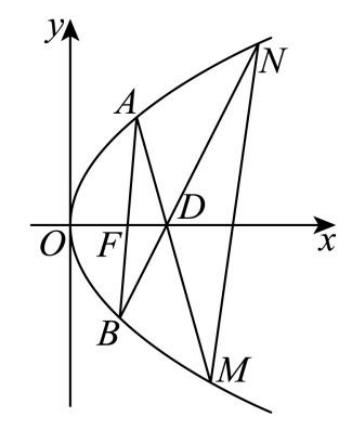
\includegraphics[width=0.2\linewidth]{bodyxb//src/qizhong202511_2.png}
            \end{center}
        \end{enumerate}
    \end{jieda}
\end{enumerate}
\subsection*{到坐标轴上点的距离最值}
\begin{enumerate}
    \item 已知点$P$在圆$x^2+(y-4)^2 = 1$上移动，点$Q$在椭圆$\dfrac{x^2}{4}+y^2 = 1$上移动，$|PQ|$的最大值为\blkda{6}.
    \begin{jieda}
        设圆心$(0, 4)$为$O$首先考虑对于一个确定的$Q$点，当$P$位于$QO$延长线于圆$x^2+(y-4)^2 = 1$的交点时，$|PQ|$最大，因此$|PQ|$的最大值即$|PO|$的最大值$+1.$

        $|PO| = \sqrt{x^2+(y-4)^2}$，代入椭圆方程，$|PO| = \sqrt{4-4y^2+(y-4)^2} = \sqrt{-3y^2-8y+20}$. 函数$f(y) = -3y^2-8y+20$的对称轴为$y = -\dfrac{4}{3}$，而$y$的取值范围是$[-1, 1]$，因此在$y = -1$处取得最值$|PO| = \sqrt{-3y^2-8y+20} \leq 5$，故$|PQ| \leq 6$
    \end{jieda}
    \item 过抛物线 ${y}^{2} = {4x}$ 上一动点 $P$ 作圆 $C : {\left( x - 3\right) }^{2} + {y}^{2} = 4$ 的两条切线,切点分别为 $A,B$ ,则四边形 ${PACB}$ 面积的最小值为\blkda{4}.
    \begin{jieda}
        由题意知 $C : {\left( x - 3\right) }^{2} + {y}^{2} = 4$ 的圆心为$(3,0)$,半径为 2.

        \begin{center}
            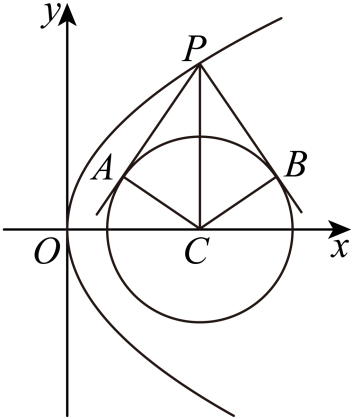
\includegraphics[width=0.2\linewidth]{bodyxb//src/paowuxianzuizhi.png}
        \end{center}
        
        如图, ${PA}\bot {AC},{PB}\bot {BC}$ ,则 ${S}_{\text{四边形 }{PACB}} = 2 \times  \dfrac{1}{2}\left| {PA}\right|  \cdot  \left| {CA}\right|  = 2\left| {PA}\right|$ .
        而 $\left| {PA}\right|  = \sqrt{{\left| PC\right| }^{2} - {\left| CA\right| }^{2}} = \sqrt{{\left| PC\right| }^{2} - 4}$ ,当 $\left| {PC}\right|$ 最小时, $\left| {PA}\right|$ 最小,则 ${S}_{\text{四边形 }{PACB}} = 2\left| {PA}\right|$ 最小;
        由于 $p$ 在抛物线 ${y}^{2} = {4x}$ 上,设 $P\left( {{t}^{2},{2t}}\right)$ .
        则 $\left| {PC}\right|  = \sqrt{{\left( {t}^{2} - 3\right) }^{2} + {\left( 2t\right) }^{2}} = \sqrt{{t}^{4} - 2{t}^{2} + 9} = \sqrt{{\left( {t}^{2} - 1\right) }^{2} + 8}$ ,
        当 ${t}^{2} = 1$ 时, ${\left( {t}^{2} - 1\right) }^{2} + 8$ 取最小值 8 ,即 $\left| {PC}\right|$ 取到最小值 $2\sqrt{2}$ ,
        则 $\left| {PA}\right|  = \sqrt{{\left| PC\right| }^{2} - 4}$ 取最小值 2 ,故 ${S}_{\text{四边形 }{PACB}} = 2\left| {PA}\right|$ 的最小值为 4.
    \end{jieda}

\end{enumerate}
\subsection*{到直线的距离}
\begin{enumerate}
    \item 求$\dfrac{x^{2}}{4}+\dfrac{y^{2}}{3} = 1$上点$P$到直线$x+y= 10$的距离的最大值.
    \begin{jieda}
        椭圆参数方程（三角代换）：$\left\{\begin{array}{l}
                x = 2cos\theta \\
                y = \sqrt{3}sin\theta
        \end{array}\right.$
        
        直线和椭圆相离，$d = \dfrac{|2cos\theta+\sqrt{3}sin\theta - 10|}{\sqrt{2}} = \dfrac{|\sqrt{7}sin(\theta+\varphi) - 10|}{\sqrt{2}} \leq \dfrac{10+\sqrt{7}}{\sqrt{2}}$
    \end{jieda}

    \item 已知 $A,B$ 分别是椭圆 $C : \dfrac{{x}^{2}}{4} + {y}^{2} = 1$ 的右顶点和上顶点, $P$ 为椭圆 $C$ 上一点,若 $\bigtriangleup  {PAB}$ 的面积是 $\sqrt{2} - 1$ ,则 $P$ 点的个数为\blkda{3}
    \begin{jieda}
        由 $C : \dfrac{{x}^{2}}{4} + {y}^{2} = 1$ 可得 $a = 2,b = 1$ ,所以 $A\left( {2,0}\right) ,B\left( {0,1}\right) ,\left| {AB}\right|  = \sqrt{5}$，直线 ${AB}$ 的方程为 $y =  - \dfrac{1}{2}x + 1$

        设过点 $P$ 与直线 ${AB}$ 平行的直线 $l : y =  - \dfrac{1}{2}x + t$ ，则直线 $l$ 与直线 ${AB}$ 的距离 $d = \dfrac{\left| t - 1\right| }{\sqrt{1 + \dfrac{1}{4}}} = \dfrac{2\sqrt{5}}{5}\left| {t - 1}\right|$. 因为 $\bigtriangleup {PAB}$ 的面积是 $\sqrt{2} - 1$，可得 ${S}_{\bigtriangleup {PAB}} = \dfrac{1}{2} \times  \left| {AB}\right|  \times  d = \dfrac{1}{2} \times  \sqrt{5} \times  \dfrac{2\sqrt{5}}{5}\left| {t - 1}\right|  = \sqrt{2} - 1$ ,解得 $t = \sqrt{2}$ 或 $t = 2 - \sqrt{2}$

        \begin{dingautolist}{172}
            \item 当 $t = \sqrt{2}$ 时,由 $\left\{  \begin{array}{l} \dfrac{{x}^{2}}{4} + {y}^{2} = 1, \\  y =  - \dfrac{1}{2}x + \sqrt{2}, \end{array}\right.$ 可得 ${\left( x - \sqrt{2}\right) }^{2} = 0$，解得 $\left\{  \begin{array}{l} x = \sqrt{2}, \\  y = \dfrac{\sqrt{2}}{2}, \end{array}\right.$ 此时 $P\left( {\sqrt{2},\dfrac{\sqrt{2}}{2}}\right)$

            \item 当 $t = 2 - \sqrt{2}$ 时,由 $\left\{  \begin{array}{l} {x}^{2} + {y}^{2} = 1, \\  y =  - \dfrac{1}{2}x + 2 - \sqrt{2}, \end{array}\right.$

            可得 ${x}^{2} + \left( {2\sqrt{2} - 4}\right) x + {10} - 8\sqrt{2} = 0$，因为 $\Delta  = {\left( 2\sqrt{2} - 4\right) }^{2} - 4\left( {{10} - 8\sqrt{2}}\right)  = {16}\left( {\sqrt{2} - 1}\right)  > 0$，此时直线 $l$ 与椭圆有 2 个交点,此时有 2 个 $P$ 点

            \ps 可以根据直线所过点$(0, 2-\sqrt2)$在椭圆内部直接判断有两个交点
        \end{dingautolist}
        所以共有 3 个 $P$ 点.
    \end{jieda} 
\end{enumerate}
\subsection*{第三定义}
\begin{enumerate}
    \item 已知 $A,B$ 两点坐标分别为 $\left( {-4,0}\right) ,\left( {4,0}\right)$ ,直线 ${AP},{BP}$ 相交于点 $P\left( {x,y}\right)$ ,且它们的斜率之积是$- \dfrac{9}{16}$ ,则代数式 $\left| {{3x} - {4y} - {24}}\right|$ 的最大值为\blkda{$24+12\sqrt{2}$}
    \begin{jieda}
        $e^2 - 1 = - \dfrac{9}{16}$，$e = \dfrac{\sqrt{7}}{4}$，$a = 4, b = 9, c = \sqrt{7}$，$\left| {{3x} - {4y} - {24}}\right| = |12cos\theta - 12sin\theta - 24| \leq 24+12\sqrt{2}$
    \end{jieda}
    \item 椭圆 $C : \dfrac{{x}^{2}}{{a}^{2}} + \dfrac{{y}^{2}}{{b}^{2}} = 1\left( {a > b > 0}\right)$ 的左顶点为 $A$ ,点 $P$ , $Q$ 均在 $C$ 上,且关于 $y$ 轴对称. 若直线 ${AP},{AQ}$ 的斜率之积为 $\dfrac{1}{4}$ ,则 $C$ 的离心率为\blkda{$\dfrac{\sqrt{3}}{2}$}
    \begin{jieda}
        根据题意可得$A(-a, 0), P(-x_0, y_0), Q(x_0, y_0)$，因此$k_{AP} = \dfrac{y_0}{a-x_0}, k_{AQ} = \dfrac{y_0}{a+x_0}$，因此$k_{AP} \cdot k_{AQ} = \dfrac{y_0^2}{a^2-x_0^2} = \dfrac{1}{4}$，即$a^2-x_0^2 = 4y_0^2$ \\
        将$P$点坐标代入椭圆方程有$\dfrac{{x_0}^{2}}{{a}^{2}} + \dfrac{{y_0}^{2}}{{b}^{2}} = 1$，即$\dfrac{a^2-4y_0^2}{a^2}+\dfrac{y_0^2}{b^2} = 1$，即$(a^2-4b^2)y_0^2 = 0$，因此必有$a^2 = 4b^2$，故$e = \dfrac{c}{a} = \sqrt{\dfrac{a^2-b^2}{a^2}} = \dfrac{\sqrt{3}}{2}$
    \end{jieda}
    \item 如图所示, $P$ 是双曲线 $\dfrac{{x}^{2}}{4} - {y}^{2} = 1$ 右支(在第一象限内)上的任意一点, ${A}_{1},{A}_{2}$ 分别是左右顶点, $O$ 是坐标原点,直线 $P{A}_{1},{PO},P{A}_{2}$ 的斜率分别为 ${k}_{1},{k}_{2},{k}_{3}$ ,则斜率之积 ${k}_{1}{k}_{2}{k}_{3}$ 的取值范围是\blkda{$\left(0, \dfrac{1}{8}\right)$}.
    \begin{center}
        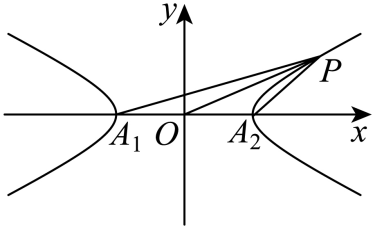
\includegraphics[width=0.2\linewidth]{bodyxb//src/shuangquxiandisandingyi.png}
    \end{center}
    \begin{jieda}
        $k_1k_2 = \dfrac{1}{4}$
    \end{jieda}
    \item 如图所示,已知 $M$ , $N$ 为双曲线 $\dfrac{{x}^{2}}{{a}^{2}} - \dfrac{{y}^{2}}{{b}^{2}} = 1$ ( $a > 0$ , $b > 0$ )上关于原点对称的两点,点 $M$ 与点 $Q$ 关于 $x$ 轴对称, $Q$为$ME$中点,直线 ${NE}$ 交双曲线右支于点 $P$ ,若 $\angle {NMP} = \dfrac{\pi }{2}$ ,则 $e =$\blkda{$\sqrt{2}$}
    \begin{center}
        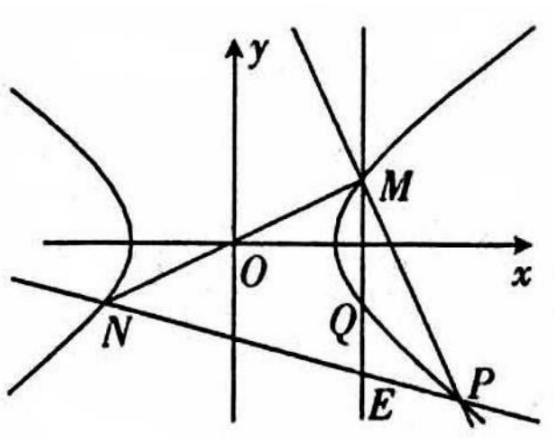
\includegraphics[width=0.2\linewidth]{bodyxb//src/disandingyi3.png}
    \end{center}
    \begin{jieda}
        设$M(x_0, y_0)$，则$N(-x_0, -y_0)$，$Q(x_0, -y_0)$，$E(x_0, -3y_0)$，故$k_{NP} = -\dfrac{y_0}{x_0}, k_{MN} = \dfrac{y_0}{x_0}, k_{MP} = -\dfrac{x_0}{y_0}$，根据第三定义有$1 = k_{NP} \cdot k_{MP} = e^2 - 1$，故$e =\sqrt{2}$
    \end{jieda}
\end{enumerate}
\subsection*{公共点的数目}
\begin{enumerate}
    \item 过点 $M\left( {2,4}\right)$ 作直线 $l$ ,与抛物线 ${y}^{2} = {8x}$ 只有一个公共点,这样的直线有\dotfill{(\kh{C})}
        \xx{0 条}{1 条}{2 条}{3 条}
    \item 曲线 ${x}^{2} - \dfrac{{y}^{2}}{4} = 1$ 是双曲线,过点 $P\left( {1,1}\right)$ 与 $C$ 恰有一个公共点且斜率存在的直线的所有可能斜率之和\blkda{$\dfrac{5}{2}$}.
    \begin{jieda}
        由题意可得 $l : y = k\left( {x - 1}\right)  + 1$ ,代入双曲线方程得 $\left( {4 - {k}^{2}}\right) {x}^{2} - 2\left( {k - {k}^{2}}\right) x - {k}^{2} + {2k} - 5 = 0$.
        
        当 $4 - {k}^{2} = 0$ ,即 $k =  \pm  2$ 时,直线 $l$ 与双曲线的渐近线平行,直线与双曲线只有一个公共点

        当 $4 - {k}^{2} \neq  0$ 时, $\Delta  = 4{\left( k - {k}^{2}\right) }^{2} - 4\left( {4 - {k}^{2}}\right) \left( {-{k}^{2} + {2k} - 5}\right)  = 0$ ,解得 $k = \dfrac{5}{2}$.

        综上,当 $k = \dfrac{5}{2}$ 或 $k =  \pm  2$ 时,直线与双曲线只有一个公共点.
    \end{jieda}
    \item 已知直线 $l$ 的方程为 $y = {kx} - 1$ ,双曲线 $C$ 的方程为 ${x}^{2} - {y}^{2} = 1$ . 若直线 $l$ 与双曲线 $C$ 的右支交于不同的两点,则实数 $k$ 的取值范围是\blkda{$\left( {1,\sqrt{2}}\right)$}
    \begin{jieda}
        \begin{enumerate}
            \item 方法1 

            联立 $\left\{  \begin{array}{l} y = {kx} - 1, \\  {x}^{2} - {y}^{2} = 1, \end{array}\right.$，整理得 $\left( {1 - {k}^{2}}\right) {x}^{2} + {2kx} - 2 = 0$，因为直线 $y = {kx} - 1$ 与双曲线 ${x}^{2} - {y}^{2} = 1$ 的右支交于不同的两点，所以 $\left\{  \begin{array}{l} 1 - {k}^{2} \neq  0, \\  \Delta  = 4{k}^{2} + 8\left( {1 - {k}^{2}}\right)  > 0, \\  \dfrac{-{2k}}{1 - {k}^{2}} > 0, \\  \dfrac{-{2}}{1 - {k}^{2}} > 0, \end{array}\right.$
            
            解得 $1 < k < \sqrt{2}$，所以实数 $k$ 的取值范围为 $\left( {1,\sqrt{2}}\right)$ .

            \item 方法2 

             $y = {kx} - 1$恒过定点$(0， -1)$，易知当$k = 1$时和双曲线的渐近线平行，而当直线斜率增大的过程中会先与双曲线右支交于两点，而后达到相切的状态，因此只需再求得相切时斜率的右边界即可.

             联立 $\left\{  \begin{array}{l} y = {kx} - 1, \\  {x}^{2} - {y}^{2} = 1, \end{array}\right.$，整理得 $\left( {1 - {k}^{2}}\right) {x}^{2} + {2kx} - 2 = 0$，令$\Delta = 0$，即$4{k}^{2} + 8\left( {1 - {k}^{2}}\right) = 0$，得到$k = \pm \sqrt{2}$，结合上述分析可知右边界为$\sqrt{2}$

             因此$k$ 的取值范围为 $\left( {1,\sqrt{2}}\right)$ .
        \end{enumerate}
    \end{jieda}

    \item 若 $P$ 是双曲线 $C : \dfrac{{x}^{2}}{{a}^{2}} - \dfrac{{y}^{2}}{{b}^{2}} = 1\left( {a > 0,b > 0}\right)$ 的渐近线上任意一点,下列正确的是\dotfill{(\kh{C})}
    \xx{存在过点 $P$ 的直线与该双曲线相切}{不存在过点 $P$ 的直线与该双曲线相切}{至多存在一条过点 $P$ 的直线与该双曲线相切}{至多存在一条过点 $P$ 的直线与该双曲线只有一个交点}
    \begin{jieda}
        当$P$为原点的时候，不存在切线，否则至多存在一条切线
    \end{jieda}
\end{enumerate}
\subsection*{中点弦}
\begin{enumerate}
    \item 已知椭圆的焦点分别为 ${F}_{1}\left( {-4,0}\right) \text{ 、 }{F}_{2}\left( {4,0}\right)$ ,过点 ${F}_{2}$ 并垂直于 $x$ 轴的直线与椭圆的一个交点为 $B$ ,且 $\left| {{F}_{1}B}\right|  + \left| {{F}_{2}B}\right|  = {10}$ . 椭圆上不同的两点 $A\left( {{x}_{1},{y}_{1}}\right) \text{ 、 }C\left( {{x}_{2},{y}_{2}}\right)$ 满足条件: $\left| {{F}_{2}A}\right| \text{ 、 }\left| {{F}_{2}B}\right| \text{ 、 }\left| {{F}_{2}C}\right|$ 成等差数列.
    \begin{enumerate*}
        \item 求该椭圆的方程；
        \item 求弦 ${AC}$ 中点的横坐标.
        \item 设弦 ${AC}$ 垂直平分线的方程为 $y = {kx} + m$ ,求 $m$ 的范围.
    \end{enumerate*}
    \begin{jieda}
        \begin{enumerate}
            \item 设椭圆的标准方程为$\dfrac{x^2}{a^2}+\dfrac{y^2}{b^2} = 1$，根据定义可知$2a = 10, a= 5$，$c = 4$，故$b = 3$，所以椭圆的标准方程$\dfrac{x^2}{25}+\dfrac{y^2}{9} = 1$
            \item 根据题意可知$|F_2B| = \dfrac{9}{5}$，因此$|F_2A| + |F_2C| = \dfrac{18}{5}$，根据椭圆第二定义可知$|F_2A| + |F_2C| = (a-ex_1)+(a-ex_2) = 2a-e(x_1+x_2) = 10 - \dfrac{4}{5}(x_1+x_2) = \dfrac{18}{5}$，因此$x_1+x_2 = 8$，故弦$AC$中点的横坐标为$4$
            \item $\dfrac{(x_1+x_2)(x_1-x_2)}{25}+\dfrac{(y_1+y_2)(y_1-y_2)}{9} = 0$

            设$AC$中点纵坐标为$y_0$，则$k_{AC} = \dfrac{y_1-y_2}{x_1-x_2} = \dfrac{x_1+x_2}{y_1+y_2} \cdot \left(-\dfrac{9}{25}\right) = -\dfrac{36}{25} \cdot \dfrac{1}{y_0}$

            故弦 ${AC}$ 垂直平分线为$y = \dfrac{25}{36}y_0(x-4)+y_0$，故$m = -\dfrac{16}{9}y_0$，而弦中点纵坐标$y_0 \in \left(-\dfrac{9}{5}, \dfrac{9}{5}\right)$，故$m \in \left(-\dfrac{16}{5}, \dfrac{16}{5}\right)$
        \end{enumerate}
    \end{jieda}
    \item 已知 $ A\left( {{x}_{1},{y}_{1}}\right) ,B\left( {{x}_{2},{y}_{2}}\right) $ 是椭圆 $ P : \dfrac{{x}^{2}}{18} + \dfrac{{y}^{2}}{9} = 1 $ 上不同的两点,线段 $ {AB} $ 的中点为 $ M\left( {2,1}\right) $.
    \begin{enumerate}
        \item 求直线 $ {AB} $ 的方程.
        \item 若线段 $ {AB} $ 的垂直平分线与椭圆 $ P $ 交于点 $ C,D $ ,问： $ A,B,C,D $ 四点是否在同一个圆上？若是,求出该圆的方程；若不是,请说明理由.
    \end{enumerate}
    \begin{jieda}
        \begin{enumerate}
            \item 因为 $ A\left( {{x}_{1},{y}_{1}}\right) ,B\left( {{x}_{2},{y}_{2}}\right) $ 是椭圆 $ P $ 上不同的两点,所以 $\left \{\begin{array}{l}
                    \dfrac{{x}_{1}^{2}}{18} + \dfrac{{y}_{1}^{2}}{9} = 1  \\
                    \dfrac{{x}_{2}^{2}}{18} + \dfrac{{y}_{2}^{2}}{9} = 1
            \end{array}\right.$.
            两式相减得 $ \dfrac{{x}_{1}^{2} - {x}_{2}^{2}}{18} + \dfrac{{y}_{1}^{2} - {y}_{2}^{2}}{9} = 0 $ ,即 $ {x}_{1}^{2} - {x}_{2}^{2} + 2\left( {{y}_{1}^{2} - {y}_{2}^{2}}\right)  = 0 $ ,
            $ \left( {{x}_{1} - {x}_{2}}\right) \left( {{x}_{1} + {x}_{2}}\right)  + 2\left( {{y}_{1} - {y}_{2}}\right) \left( {{y}_{1} + {y}_{2}}\right)  = 0. $
            因为线段 $ {AB} $ 的中点为 $ M\left( {2,1}\right) $ ,所以 $ {x}_{1} + {x}_{2} = 4,{y}_{1} + {y}_{2} = 2 $ .
            所以 $ 4\left( {{x}_{1} - {x}_{2}}\right)  + 4\left( {{y}_{1} - {y}_{2}}\right)  = 0 $ .
            当 $ {x}_{1} = {x}_{2} $ 时,由上式知 $ {y}_{1} = {y}_{2} $ ,故点 $ A,B $ 重合,与已知矛盾,因此 $ {x}_{1} \neq  {x}_{2} $ ,所以 $ \dfrac{{y}_{1} - {y}_{2}}{{x}_{1} - {x}_{2}} =  - 1 $ .
            所以直线 $ {AB} $ 的方程为 $ y - 1 =  - \left( {x - 2}\right) $ ,即 $ x + y - 3 = 0 $ .
            所以所求直线 $ {{AB}} $ 的方程为 $ x + y - 3 = 0 $ .
            \item 
            根据圆心位于中垂线$CD$上，因此可以考虑求出中垂线上的弦的中点$E$坐标后计算$EA$的距离，判断其是否等于$EC$即可. 
            
            由于直线 $ {AB} $ 的方程为 $ x + y - 3 = 0 $ ,则线段 $ {AB} $ 的垂直平分线 $ {CD} $ 的方程为 $ y - 1 = x - 2 $ ,即 $ x - y - 1 = 0 $ .
            由 $ \left\{  \begin{array}{l} x + y - 3 = 0, \\  \dfrac{{x}^{2}}{18} + \dfrac{{y}^{2}}{9} = 1, \end{array}\right. $ 得 $ A\left( {0,3}\right) ,B\left( {4, - 1}\right) $ ,由 $ \left\{  \begin{array}{l} x - y - 1 = 0, \\  \dfrac{{x}^{2}}{18} + \dfrac{{y}^{2}}{9} = 1, \end{array}\right. $ ,消去 $ y $ 得 $ 3{x}^{2} - {4x} - {16} = 0 $ .
            
            设 $ C\left( {{x}_{3},{y}_{3}}\right) ,D\left( {{x}_{4},{y}_{4}}\right) $ ,则 $ {x}_{3} + {x}_{4} = \dfrac{4}{3},{x}_{3}{x}_{4} =  - \dfrac{16}{3} $ .
            所以线段 $ {CD} $ 的中点 $ E $ 的横坐标为 $ {x}_{E} = \dfrac{{x}_{3} + {x}_{4}}{2} = \dfrac{2}{3} $ ,纵坐标 $ {y}_{E} = {x}_{E} - 1 =  - \dfrac{1}{3} $，所以 $ E\left( {\dfrac{2}{3}, - \dfrac{1}{3}}\right)$
            
            $\left| {CD}\right|  = \sqrt{\left( {1 + 1}\right) \left\lbrack  {{\left( {x}_{3} + {x}_{4}\right) }^{2} - 4{x}_{3}{x}_{4}}\right\rbrack  } = \sqrt{2\left\lbrack  {{\left( \dfrac{4}{3}\right) }^{2} - 4 \times  \left( {-\dfrac{16}{3}}\right) }\right\rbrack  } = \dfrac{4\sqrt{26}}{3} $ .
            因为 $\left| {EB}\right|  = \left| {EA}\right|  = \sqrt{{\left( \dfrac{2}{3}\right) }^{2} + {\left( -\dfrac{1}{3} - 3\right) }^{2}} = \dfrac{2\sqrt{26}}{3} = \dfrac{1}{2}\left| {CD}\right|$ ,所以 $ A,B,C,D $ 四点在同一个圆上,此圆的圆心为点 $ E $ ,半径为 $ \dfrac{2\sqrt{26}}{3} $ ,其方程为
            $ {\left( x - \dfrac{2}{3}\right) }^{2} + {\left( y + \dfrac{1}{3}\right) }^{2} = \dfrac{104}{9}. $
        \end{enumerate}
    \end{jieda}
    \item 已知双曲线 $C : \dfrac{{x}^{2}}{{a}^{2}} - \dfrac{{y}^{2}}{{b}^{2}} = 1\left( {a > 0,b > 0}\right)$ 过点 $\left( {2\sqrt{2},1}\right)$ ,渐近线方程为 $y =  \pm  \dfrac{1}{2}x$ ,直线 $l$ 是双曲线 $C$ 右支的一条切线,且与 $C$ 的渐近线交于 $A,B$ 两点.
    \begin{enumerate}
        \item 求双曲线 $C$ 的方程
        \item 设点 $A,B$ 的中点为 $M$ ,求点 $M$ 到 $y$ 轴的距离的最小值.
    \end{enumerate}
    \begin{jieda}
        \begin{enumerate}
            \item 题设可知 $\left\{  \begin{array}{l} \dfrac{8}{{a}^{2}} - \dfrac{1}{{b}^{2}} = 1, \\  \dfrac{b}{a} = \dfrac{1}{2}, \end{array}\right.$，解得 $\left\{  \begin{array}{l} a = 2, \\  b = 1, \end{array}\right.$，因此$C : \dfrac{{x}^{2}}{4} - {y}^{2} = 1$ .
            \item 
            \begin{dingautolist}{172}
                \item 当直线 $l$ 的斜率不存在时,则直线 $l : x = 2$，易知点 $M$ 到 $y$ 轴的距离为 ${x}_{M} = 2$
                \item 当直线 $l$ 的斜率存在时，设 $l : y = {kx} + m\left( {k \neq   \pm  \dfrac{1}{2}}\right) ,A\left( {{x}_{1},{y}_{1}}\right) ,B\left( {{x}_{2},{y}_{2}}\right)$ ,
                
                联立 $\left\{  \begin{array}{l} \dfrac{{x}^{2}}{4} - {y}^{2} = 1, \\  y = {kx} + m, \end{array}\right.$ 整理得 $\left( {4{k}^{2} - 1}\right) {x}^{2} + {8kmx} + 4{m}^{2} + 4 = 0$ ,
                
                $\Delta  = {64}{k}^{2}{m}^{2} - {16}\left( {4{k}^{2} - 1}\right) \left( {{m}^{2} + 1}\right)  = 0$，整理得 $4{k}^{2} = {m}^{2} + 1$ ,
                
                联立 $\left\{  \begin{array}{l} \dfrac{{x}^{2}}{4} - {y}^{2} = 0, \\  y = {kx} + m, \end{array}\right.$ 整理得 $\left( {4{k}^{2} - 1}\right) {x}^{2} + {8kmx} + 4{m}^{2} = 0$ ,
                
                则 ${x}_{1} + {x}_{2} =  - \dfrac{8km}{4{k}^{2} - 1} =  - \dfrac{8km}{{m}^{2}} =  - \dfrac{8k}{m}$ ,则 ${x}_{M} = \dfrac{{x}_{1} + {x}_{2}}{2} =  - \dfrac{4k}{m}$
                
                则 ${x}_{M}^{2} = \dfrac{{16}{k}^{2}}{{m}^{2}} = 4 + \dfrac{4}{{m}^{2}} > 4$，即 $|{x}_{M}| > 2$（事实上$x_M$为正），此时点 $M$ 到 $y$ 轴的距离大于 2 .
            \end{dingautolist}
            综上所述，点 $M$ 到 $y$ 轴的最小距离为 2 .
        \end{enumerate}
    \end{jieda}
    \item 设直线 $l$ 与抛物线 ${y}^{2} = {4x}$ 相交于 $A\text{ 、 }B$ 两点,与圆 ${\left( x - 5\right) }^{2} + {y}^{2} = {r}^{2}\left( {r > 0}\right)$ 相切于点 $M$ , 且 $M$ 为线段 ${AB}$ 的中点,若这样的直线 $l$ 恰有 4 条,则 $r$ 的取值范围是\blkda{$(2, 4)$}.
    \begin{jieda}
        数形结合可知有两条切线为垂直于$x$轴的切线

        设斜率存在时$M(x_0, y_0)$，因此对应的切线$AB$为$(x-5)(x_0 - 5)+yy_0 = r^2$，设$A(x_1, y_1), B(x_2, y_2)$，则有$\left\{\begin{array}{l}
             y_1^2 = 4x_1 \\
             y_2^2 = 4x_2
        \end{array}\right.$，两者作差有$(y_1^2 - y_2^2) = 4(x_1-x_2)$即$(y_1+y_2)(y_1 - y_2) = 4(x_1-x_2)$，故$k_{AB} = \dfrac{4}{y_1+y_2} = \dfrac{2}{y_0}$，根据方程$(x-5)(x_0 - 5)+yy_0 = r^2$可知$k_{AB} = \dfrac{5-x_0}{y_0}$，因此$x_0 = 3$

        故当圆上存在横坐标为$3$的点时会出现另外两条切线，但根据图象可知圆上横坐标为$3$的点应在抛物线内部才可以，即$r \in (2, 4)$
    \end{jieda}
\end{enumerate}
\subsection*{双曲线的中点弦存在性问题}
\begin{enumerate}
    \item 已知双曲线 ${C}$ 的方程为 ${x}^{2} - \dfrac{{y}^{2}}{2} = 1$ ,试判断过点 $P\left( {1,1}\right)$ 能否作一条直线 $l$ 与双曲线交于 $A\text{ 、 }B$ 两点,且 $P$ 为 ${AB}$ 的中点,并说明理由.
    \begin{jieda}
        设双曲线上两点$A(x_1, y_1), B(x_2, y_2)$，$P$ 为 ${AB}$ 的中点，则有$\left\{\begin{array}{l}
                {x_1}^{2} - \dfrac{{y_1}^{2}}{2} = 1  \\
                {x_2}^{2} - \dfrac{{y_2}^{2}}{2} = 1
        \end{array}\right.$，两式作差有$(x_1+x_2)(x_1-x_2) - \dfrac{(y_1+y_2)(y_1-y_2)}{2} = 0$，根据$P$为中点有$x_1+x_2 = 2, y_1+y_2 = 2$，故$2(x_1-x_2) - (y_1-y_2) = 0$，即$k_{AB} = 2$，故$AB: y = 2x-1$

        联立直线和双曲线方程有$\left\{\begin{array}{l}
                y = 2x-1  \\
                {x}^{2} - \dfrac{{y}^{2}}{2} = 1
        \end{array}\right.$，消去$y$可得$2x^2-(2x-1)^2 = 2$，即$-2x^2+4x-3=0$，方程无解，故不存在.
    \end{jieda}

    \item 设 $A,B$ 为双曲线 ${x}^{2} - \dfrac{{y}^{2}}{9} = 1$ 上两点,下列四个点中,可为线段 ${AB}$ 中点的是\dotfill{(\kh{D})}
    \xx{$(1,1)$}{$(-1,2)$}{$(1,3)$}{$(-1,-4)$}
    \begin{jieda}
        弦中点不会位于双曲线和渐近线中间的区域. 不利用结论可以点差法逐一求出直线方程检验.
    \end{jieda}
    
    \item 已知双曲线 $C : \dfrac{{x}^{2}}{{a}^{2}} - \dfrac{{y}^{2}}{{b}^{2}} = 1\left( {a > 0,b > 0}\right)$ ,若双曲线上不存在以点$(2a, a)$为中点的弦,则双曲线离心率 $e$ 的取值范围是\blkda{$\left\lbrack  {\dfrac{\sqrt{5}}{2},\dfrac{2\sqrt{3}}{3}}\right\rbrack$}
    \begin{jieda}
        $\dfrac{4{a}^{2}}{{a}^{2}} - \dfrac{a^{2}}{{b}^{2}} \in [0, 1]$，即$\dfrac{a^{2}}{{b}^{2}} \in [3, 4]$，故$e \in \left\lbrack  {\dfrac{\sqrt{5}}{2},\dfrac{2\sqrt{3}}{3}}\right\rbrack$
    \end{jieda}
\end{enumerate}
\subsection*{蒙日圆与最值问题转化}
\begin{enumerate}
    \item 证明：椭圆$\dfrac{x^2}{a^2}+\dfrac{y^2}{b^2} = 1 (a>b>0)$中任意两条互相垂直的切线的交点都在同一个圆上，并求圆的方程.
    \begin{jieda}
        设椭圆$\dfrac{x^2}{a^2}+\dfrac{y^2}{b^2} = 1 (a>b>0)$左焦点为$F_1$，右焦点为$F_2$，设过点 $p\left( {{x}_{0},{y}_{0}}\right)$ 的两切线$l_1, l_2$

        做$F_1$关于$l_1$的对称点$F_1'$，关于$l_2$的对称点$F_1''$，则$\triangle F_2F_1'F_1''$为腰长$2a$的等腰三角形，$\triangle F_1F_1'F_1''$为直角三角形，故$F_1P = F_1'P$，故根据勾股定理有$|F_2P|^2 + |F_1'P|^2 = 4a^2$，$|F_2P|^2 + |F_1P|^2 = 4a^2$因此$|PO|^2 = \left|\dfrac{\vv{F_1P}+\vv{F_2P}}{2}\right|^2 = \dfrac{|F_1P|^2+|F_2P|^2 + 2\vv{F_1P} \cdot \vv{F_2P}}{4} = a^2 + \dfrac{|PO|^2 - c^2}{2}$，故$|PO|^2 = a^2+b^2$  
    \end{jieda}
     \item 法国著名数学家蒙日发现椭圆 $\dfrac{{x}^{2}}{{a}^{2}} + \dfrac{{y}^{2}}{{b}^{2}} = 1\left( {a > b > 0}\right)$ 的两条相互垂直的切线的交点的轨迹是圆,且方程为 ${x}^{2} + {y}^{2} = {a}^{2} + {b}^{2}$ ,这个圆被称为 “蒙日圆”. 已知椭圆 $C : \dfrac{{x}^{2}}{m} + \dfrac{{y}^{2}}{4} = 1$ 的焦点在 $x$ 轴上, $A,B$ 为椭圆 $C$ 上任意两点,动点 $P$ 在直线 $x - \sqrt{3}y - 4\sqrt{3} = 0$ 上. 若 $\angle {APB}$ 恒为锐角, 则椭圆 $C$ 的离心率的取值范围为\blkda{$\left( {0,\dfrac{\sqrt{2}}{2}}\right)$}
    \begin{jieda}
        由题意知 $m > 4$ ,圆 ${x}^{2} + {y}^{2} = m + 4$ 为椭圆 $C : \dfrac{{x}^{2}}{m} + \dfrac{{y}^{2}}{4} = 1$ 的“蒙日圆”,
        
        如图,因为 $A,B$ 为椭圆 $C$ 上任意两点,动点 $P$ 满足 $\angle {APB}$ 恒为锐角,
        
        则点 $P$ 在圆 ${x}^{2} + {y}^{2} = m + 4$ 外,又动点 $P$ 在直线 $x - \sqrt{3}y - 4\sqrt{3} = 0$ 上,
        
        则直线 $x - \sqrt{3}y - 4\sqrt{3} = 0$ 与圆 ${x}^{2} + {y}^{2} = m + 4$ 相离,
        
        所以 $\dfrac{\left| -4\sqrt{3}\right| }{\sqrt{{1}^{2} + {\left( -\sqrt{3}\right) }^{2}}} > \sqrt{m + 4}$ ,得 $m < 8$ ,所以 $4 < m < 8$ ,
        
        则 $\dfrac{{c}^{2}}{{a}^{2}} = 1 - \dfrac{{b}^{2}}{{a}^{2}} = 1 - \dfrac{4}{m} \in  \left( {0,\dfrac{1}{2}}\right)$ ,又椭圆的离心率大于零,
        
        则椭圆 $C$ 的离心率的取值范围是 $\left( {0,\dfrac{\sqrt{2}}{2}}\right)$ .
        
        \begin{center}
        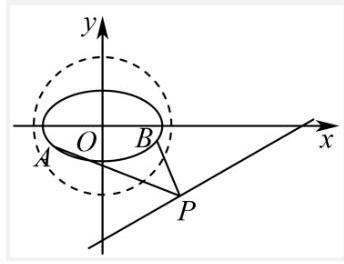
\includegraphics[width=0.2\textwidth]{bodyxb/src/bo_d3jiq7ref24c73cufkeg_0_240_1737_344_264_0.jpg}
        \end{center}
    \end{jieda}
    
    \item 加斯帕尔·蒙日是 $18\~19$ 世纪法国著名的几何学家, 他在研究时发现: 椭圆的任意两条互相垂直的切线的交点都在同一个圆上, 其圆心是椭圆的中心, 这个圆被称为 “蒙日圆”. 已知椭圆 $C : \dfrac{{x}^{2}}{9} + \dfrac{{y}^{2}}{{b}^{2}} = 1\left( {{b}^{2} < 9}\right)$ ,若直线 $l : {4x} - {3y} + {20} = 0$ 上存在点 $P$ ,过 $P$ 可作 $C$ 的两条互相垂直的切线,则椭圆离心率的取值范围是\blkda{$\left( {0,\dfrac{\sqrt{2}}{3}}\right\rbrack$}
    \begin{jieda}
        由题可知,点 $P$ 在椭圆的蒙日圆上,又因为点 $P$ 在直线上,所以,问题转化为直线和蒙日圆有公共点.
    
        蒙日圆方程为 ${x}^{2} + {y}^{2} = {b}^{2} + 9$ , 因此,需满足圆心到直线 ${4x} - {3y} + {20} = 0$ 的距离不大于半径，即 $\dfrac{20}{5} \leq  \sqrt{{b}^{2} + 9}$ ,所以 ${b}^{2} \geq  7$ ,所以椭圆离心率 ${e}^{2} = 1 - \dfrac{{b}^{2}}{9} \leq  \dfrac{2}{9}$ ,所以 $0 < e \leq  \dfrac{\sqrt{2}}{3}$ .
    \end{jieda}

    \item 已知 $P\text{、}Q$ 是曲线 $\Gamma$ 上两点,若对于平面内任意不在曲线 $\Gamma$ 上的 $M$ 点,使得曲线 $\Gamma$ 上存在点 $P$ 和点 $Q$ 使得 ${MP}\bot {MQ}$ ,则称曲线 $\Gamma$ 是“ ${YY}$ 曲线”. 现有如下两个命题：\ding{172}任意椭圆都是“ ${YY}$ 曲线”；\ding{173}任意双曲线都是“ ${YY}$ 曲线”. 则\dotfill{(\kh{D})}
    \xx{\ding{172} 是真命题， \ding{173} 是真命题}{\ding{172} 是真命题， \ding{173} 是假命题}{\ding{172} 是假命题， \ding{173} 是真命题}{\ding{172} 是假命题， \ding{173} 是假命题}
\end{enumerate}
\subsection*{椭圆和双曲线拼接}
\begin{enumerate}
    \item 已知曲线 $C : \dfrac{x\left| x\right| }{{a}^{2}} - \dfrac{y\left| y\right| }{{b}^{2}} = 1$ ,下列叙述中错误的是\dotfill{(\kh{C})}
    \xx{垂直于 $x$ 轴的直线与曲线 $C$ 只有一个交点}{直线 $y = {kx} + m\left( {k,m \in  \mathbf{R}}\right)$ 与曲线 $C$ 最多有三个交点}{曲线 $C$ 关于直线 $y =  - x$ 对称}{若 ${P}_{1}\left( {{x}_{1},{y}_{1}}\right) \text{ 、 }{P}_{2}\left( {{x}_{2},{y}_{2}}\right)$ 为曲线 $C$ 上任意两点,则有 $\dfrac{{y}_{1} - {y}_{2}}{{x}_{1} - {x}_{2}} > 0$}
    \begin{jieda}
        数形结合可知
    \end{jieda}
    \item 方程 $\dfrac{x\left| x\right| }{16} + \dfrac{y\left| y\right| }{9} =  - 1$ 的曲线即为函数 $y = f\left( x\right)$ 的图象,对于函数 $y = f\left( x\right)$ ,有如下结论:\ding{172} $f\left( x\right)$ 在 $\mathbf{R}$ 上单调递减；\ding{173}函数 $F\left( x\right)  = {4f}\left( x\right)  + {3x}$ 不存在零点；\ding{174}函数 $y = f\left( x\right)$ 的值域是 $\mathbf{R}$ ；\ding{175}若函数 $g\left( x\right)$ 和 $f\left( x\right)$ 的图象关于原点对称,则 $y = g\left( x\right)$ 由方程 $\dfrac{y\left| y\right| }{16} + \dfrac{x\left| x\right| }{9} = 1$ 确定. 其中所有正确的命题序号是\dotfill{(\kh{D})}
    \xx{\ding{172}\ding{174}}{\ding{172}\ding{175}}{\ding{172}\ding{174}\ding{175}}{\ding{172}\ding{173}\ding{174}}

    \begin{jieda}
        分类讨论可知该方程即$\left\{\begin{array}{ll}
                \dfrac{x^2}{16}-\dfrac{y^2}{9} = 1, & (x, y)\text{在第二象限}  \\
                \dfrac{x^2}{16}+\dfrac{y^2}{9} = 1, & (x, y)\text{在第三象限}  \\
                -\dfrac{x^2}{16}+\dfrac{y^2}{9} = 1, & (x, y)\text{在第四象限}
        \end{array}\right.$，为一段连续的曲线
        \begin{dingautolist}{172}
            \item 结合图像易知$f(x)$单调递减
            \item $f(x)$在二四象限的两段双曲线的渐近线为$y = -\dfrac{3}{4}x$，$F\left( x\right)  = {4f}\left( x\right)  + {3x}$ 不存在零点即$y = f(x) + \dfrac{3}{4}x$没有零点，即$y = f(x)$与$y = -\dfrac{3}{4}x$没有交点，结合图像可知正确
            \item 结合图像易知函数 $y = f\left( x\right)$ 的值域是 $\mathbf{R}$
            \item $y = g\left( x\right)$ 应由方程 $\dfrac{y\left| y\right| }{9} + \dfrac{x\left| x\right| }{16} = 1$ 确定，故错误
        \end{dingautolist}
    \end{jieda}
\end{enumerate}
\subsection*{圆锥曲线与重心}
\begin{enumerate}
    \item 设抛物线 ${x}^{2} = {4y}$ 的焦点为 ${F}$ ,点 $A\text{ 、 }B\text{ 、 }C$ 在抛物线上,若 $\vv{FA} + \vv{FB} + \vv{FC} = \vv{0}$ , 则 $\left| \vv{FA}\right|  + \left| \vv{FB}\right|  + \left| \vv{FC}\right|  =$ \blkda{6}.
    \begin{jieda}
        $p = 2, F$为$\triangle ABC$重心，$y_A+y_B+y_C = 3y_F = 3$，$\left| \vv{FA}\right|  + \left| \vv{FB}\right|  + \left| \vv{FC}\right|  = y_A+y_B+y_C + \dfrac{3p}{2} = 3+3 = 6$
    \end{jieda}
    \item 已知 $A,B,C$ 是椭圆 $\dfrac{{x}^{2}}{12} + \dfrac{{y}^{2}}{4} = 1$ 上三个不同的点, $\bigtriangleup  {ABC}$ 的重心为原点 $O$ ,那么 $\bigtriangleup  {ABC}$ 的面积是\blkda{9}.
    \begin{jieda}
        设$A(2\sqrt{3}cos\alpha, 2sin\alpha)$，$B(2\sqrt{3}cos\beta, 2sin\beta)$，因为$O$是$\bigtriangleup  {ABC}$ 的重心，所以$C(-2\sqrt{3}(cos\alpha + cos\beta), -2(sin\alpha+sin\beta))$，因为$C$在椭圆上，所以$(cos\alpha + cos\beta)^2+(sin\alpha+sin\beta)^2 = 1$，即$1+2cos(\alpha-\beta) = 0$，故$cos(\alpha - \beta) = -\dfrac{1}{2}$

        $S = 3 \times \dfrac{1}{2} \times 4\sqrt{3}|cos\alpha sin\beta - sin\alpha cos\beta| = 6\sqrt{3}|sin(\beta-\alpha)| = 6\sqrt{3} \times \dfrac{\sqrt{3}}{2} = 9$

    \end{jieda}
    \item 已知过原点的直线 $l$ 交椭圆 $\dfrac{{x}^{2}}{9} + \dfrac{{y}^{2}}{4} = 1$ 于 $P,Q$ 两点,椭圆右顶点为 $A,\bigtriangleup {APQ}$ 重心为 $G$ , $\left| {GA}\right|  + \left| {GP}\right|  + \left| {GQ}\right|$ 的取值范围是\blkda[3]{$[2\sqrt{5}+2, 8)$}.
    \begin{jieda}
        $A(3, 0)$，根据重心性质可知$G(1, 0)$，设$P(x_0, y_0)$，则$Q(-x_0, -y_0)$，故$|GP|+|GQ| = \sqrt{(x_0-1)^2+y_0^2}+\sqrt{(x_0+1)^2+y_0^2}$

        当$\sqrt{(x_0-1)^2+y_0^2}+\sqrt{(x_0+1)^2+y_0^2}$等于大于2的常值时，$(x_0, y_0)$在以$(1, 0), (-1, 0)$为焦点的椭圆$\dfrac{x^2}{k}+\dfrac{y^2}{k-1} = 1$上，故数形结合可知$k \in [5, 9)$（$k = 9$时$Q$与$A$重合），即$\sqrt{(x_0-1)^2+y_0^2}+\sqrt{(x_0+1)^2+y_0^2} \in [2\sqrt{5}, 6)$

        $\left| {GA}\right|  + \left| {GP}\right|  + \left| {GQ}\right| \in [2\sqrt{5}+2, 8)$
    \end{jieda}
\end{enumerate}
\subsection*{抛物线焦点弦是准线上一点的切点弦}
\begin{enumerate}
    \item 已知点 $M\left( {-1,1}\right)$ 和抛物线 $C : {y}^2 = {4x}$ ,过 $C$ 的焦点且斜率为 $k$ 的直线与 $C$ 交于 $A,B$ 两点. 若 $\angle {AMB} = {90}^{ \circ  }$ , 则 $k =$ \blkda{2}

    \item 过点 $M\left( {-1,m}\right)$ 作抛物线 $C : {y}^2 = {2px},\left( {p > 0}\right)$ 的两条切线,切点分别为 $A\left( {{x}_1,{y}_1}\right)$ 和 $B\left( {{x}_2,{y}_2}\right)$ ,又直线 ${AB}$ 经过抛物线 $C$ 的焦点 $F$ ，那么 $\dfrac{{y}_1{y}_2}{{k}_{MA}{k}_{MB}} =$ \blkda{4}

    \item 已知抛物线$\Gamma: y^2 = 8x$的焦点为$F$，经过$F$的直线$l$与抛物线$\Gamma$交于$A, B$两点，设$M$在抛物线的准线上，若$\triangle MAB$为等腰直角三角形，则$|AB| = $\blkda{$8$或$\dfrac{25}{2}$}
    \begin{jieda}
        \begin{dingautolist}{172}
            \item 若$M$是直角顶点，则$AB$为通径满足要求，$|AB| = 8$
            \item 若$A$为直角顶点，则过$A,B$做准线的垂线$AA', BB'$，过$A$做直线$BB'$垂线，垂足为$H$，则$\triangle AA'M \cong \triangle AHB$
            
            设$|AF| = x, |BF| = y$，则$|AH| = x, |BH| = x-y$，因此$\dfrac{x}{y} = 4$，根据焦半径公式可知$\dfrac{p}{1-cos\alpha} = \dfrac{4p}{1+cos\alpha}$，故$cos\alpha = \dfrac{3}{5}$，$|AB| = \dfrac{2p}{sin^2\alpha} = \dfrac{25}{2}$
        \end{dingautolist}
    \end{jieda}
\end{enumerate}
\subsection*{斜椭圆}
\begin{enumerate}
    \item 已知复数 ${z}_1,{z}_2$ 满足 $\left| {{z}_1 + \sqrt{3} - {i}}\right|  + \left| {{z}_1 - \sqrt{3} + {i}}\right|  = 2\sqrt{5},{z}_2 = 2 + 2\sqrt{3}{i}$ ,(其中 ${i}$ 是虚数单位),则 $\left| {{z}_1 - {z}_2}\right|$ 的最小值为\blkda{3}
    \begin{jieda}
        设复数 ${z}_1$，${z}_2 = 2 + 2\sqrt{3}{i}$，$- \sqrt{3} + {i}$，$\sqrt{3} - {i}$ 在复平面内对应的点分别为 ${Z}_1\left( {x,y}\right) ,{Z}_2\left( {2,2\sqrt{3}}\right) ,{F}_1\left( {-\sqrt{3},1}\right) ,{F}_2\left( {\sqrt{3}, - 1}\right)$ 
        
        由题意可知: $\left| {{Z}_1{F}_1}\right|  + \left| {{Z}_1{F}_2}\right|  = 2\sqrt{5} > 4 = \left| {{F}_1{F}_2}\right|$，故${Z}_1$ 的轨迹表示焦点分别为 ${F}_1\left( {-\sqrt{3},1}\right) ,{F}_2\left( {\sqrt{3}, - 1}\right)$ 的椭圆,

        \begin{center}
        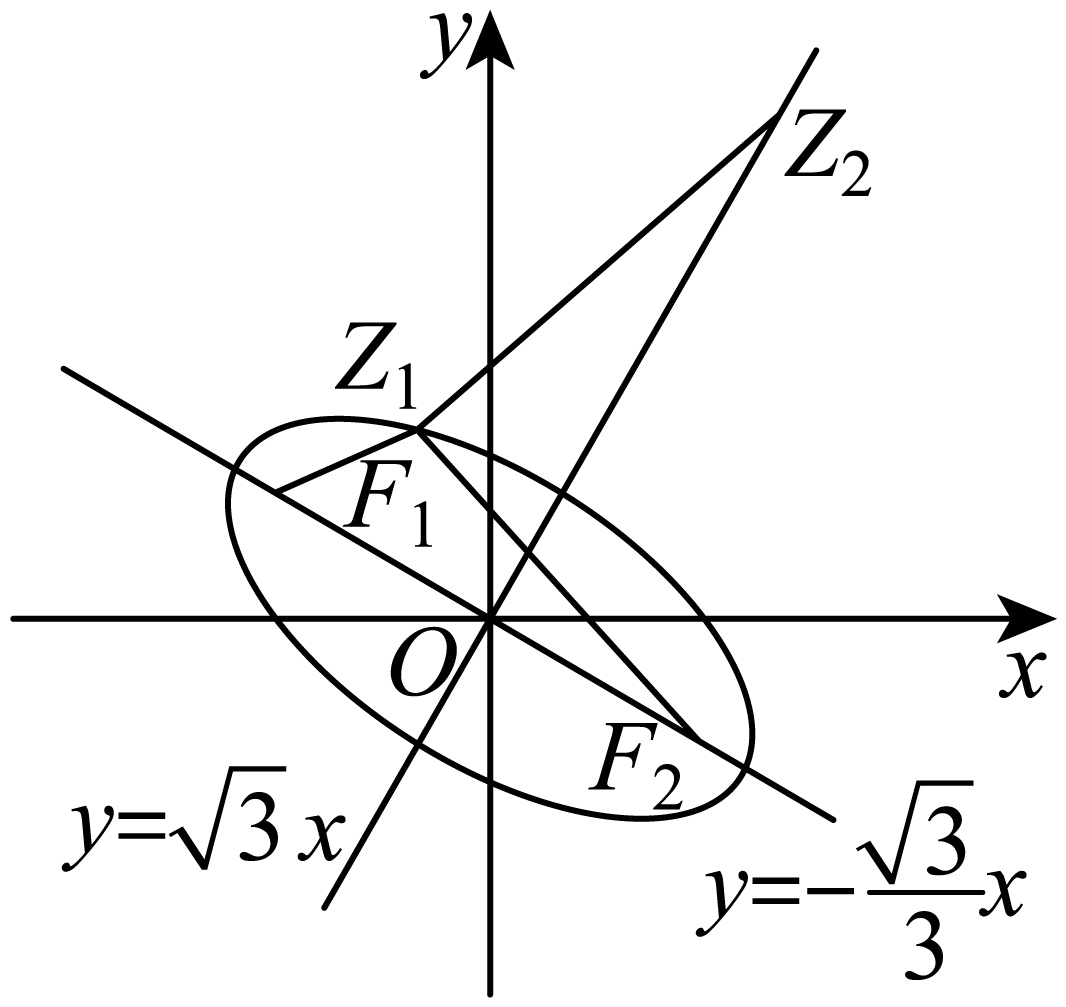
\includegraphics[width=0.2\textwidth]{bodyxb/src/0_13_153_215_205_0.png}
        \end{center}

        则长半轴长为 $a = \sqrt{5}$ ,半焦距 $c = 2$ ,短半轴长为 $b = \sqrt{{a}^2 - {c}^2} = 1$ ,

        且该椭圆的长轴所在直线为 $y =  - \dfrac{\sqrt{3}}{3}x$ ,短轴所在直线为 $y = \sqrt{3}x$.

        ${Z}_2$ 在 $y = \sqrt{3}x$ 上,且 $\left| {O{Z}_2}\right|  = 4$，若使得 $\left| {{z}_1 - {z}_2}\right|$ 最小,则需 $\left| {{Z}_1{Z}_2}\right|$ 取得最小值，即点 ${Z}_1$ 为第一象限内的短轴端点,此时 $\left| {{z}_1 - {z}_2}\right|  = \left| {O{Z}_2}\right|  - 1 = 3$ .
    \end{jieda}
    \item 已知复数 $z$ 满足 $\left| {z - 4{i}}\right|  + \left| {z + 5}\right|  = \sqrt{41}$ ( ${i}$ 为虚数单位)，则 $\left| {z - {i}}\right|$ 的最小值是\blkda{$\dfrac{15\sqrt{41}}{41}$}.
    \begin{jieda}
        \ps 不符合椭圆定义，轨迹是线段
    \end{jieda}
    \item 著名物理学家、数学家阿基米德利用 “逼近法”,得到椭圆的面积除以圆周率 $\pi$ 等于椭圆的长半轴长与短半轴长的乘积. 已知平面内,椭圆 $C : \dfrac{{x}^2}{9} + \dfrac{{y}^2}{{b}^2} = 1\left( {0 < b < 3}\right)$ 经过平移和旋转后，能得到以 $O\left( {0,0}\right)$ 为一个焦点，且过点 $A\left( {3,4}\right)$ 的椭圆 ${C}^{\prime }$ ，则椭圆 $C$ 面积的最大值为\blkda{$3\sqrt{5}\pi$.}
    \begin{jieda}
        椭圆面积公式$S = \pi ab$，$a = 3$，故应使得$b$尽可能大，$c$尽可能小，$e$尽可能小.

        问题转化为已知椭圆存在一个长为$5$的焦半径，一个长为$1$的焦半径，根据焦半径公式$5 = a + ex_0$可知当取到长轴顶点时可使$e$取最小，此时$c = 2$，$b = \sqrt{5}$，$S = 3\sqrt{5}\pi$.
    \end{jieda}
\end{enumerate}
\subsection*{圆锥曲线定义识别}
\begin{enumerate}
    \item 已知向量$\vv{e_1}, \vv{e_2}$是相互垂直的单位向量，$\vv{a}$是平面内的向量，若对任意的$\lambda \in \mathbf{R}$，都有$|\vv{a}+\lambda \vv{e_1}| \geq |\vv{a} - \vv{e_2}|$，且存在$\lambda$使得等号成立，则$|\vv{e_1}+3\vv{e_2}-\vv{a}| + |\vv{a} - \vv{e_2}|$的最小值为\blkda{3}
    \begin{jieda}
        $|\vv{a}+\lambda \vv{e_1}| \geq |\vv{a} - \vv{e_2}|$恒成立，且可以取等即在共起点的情况下，$\vv{a}$终点到过起点$\vv{e_1}$所在的直线的距离等于$\vv{a}$与$\vv{e_2}$终点的距离（符合抛物线的定义） \\
        设$\vv{e_1} = (1, 0), \vv{e_2} = (0, 1), \vv{a} = (x, y)$，则有$y^2 = x^2 + (y-1)^2$，即$y = \dfrac{x^2+1}{2}$，故$\vv{a}$的终点在抛物线上. \\
        $|\vv{e_1}+3\vv{e_2}-\vv{a}| + |\vv{a} - \vv{e_2}|$即$\vv{a}$的终点到$\vv{e_1}+3\vv{e_2}$终点距离与$\vv{a}$终点到$\vv{e_2}$终点距离之和，设其为$s$，$s = \sqrt{(x-1)^2+(y-3)^2} + \sqrt{x^2 + (y-1)^2} = \sqrt{(x-1)^2+(y-3)^2}+\sqrt{y^2} \geq 3$
        （\ps $\vv{a}$终点到$\vv{e_2}$终点距离即抛物线上点到焦点的距离，等于抛物线上点到准线的距离，故当$\vv{a}$终点位于$\vv{e_1}+3\vv{e_2}$终点到准线的垂线与抛物线交点，即$\vv{a} = (1,1)$，时$s$最小为3）
    \end{jieda}

    \item (2025$\cdot$宝山区一模$\cdot$16)设 $\bigtriangleup {A}_{n}{B}_{n}{C}_{n}$ 的三边长分别为 ${a}_{n}$ 、 ${b}_{n}$ 、 ${c}_{n}$ ，面积为 ${S}_{n}$ ( $n$ 为正整数). 若 ${b}_{1} - {c}_{1} = \dfrac{1}{2}{a}_{1}$ ,其中 ${c}_{1} > \dfrac{1}{4}{a}_{1},{a}_{n + 1} = {a}_{n},{b}_{n + 1} = {c}_{n} + \dfrac{1}{4}{a}_{n},{c}_{n + 1} = {b}_{n} + \dfrac{1}{4}{a}_{n}$ ,则 \dotfill{(\kh{B})}
    \xx{$\left\{  {S}_{n}\right\}$ 为严格减数列}{$\left\{  {S}_{n}\right\}$ 为严格增数列}{$\left\{  {S}_{{2n} - 1}\right\}$ 为严格增数列, $\left\{  {S}_{2n}\right\}$ 为严格减数列}{$\left\{  {S}_{{2n} - 1}\right\}$ 为严格减数列, $\left\{  {S}_{2n}\right\}$ 为严格增数列}
    \begin{jieda}
        由已知 ${a}_{n + 1} = {a}_{n}$ ,即 $\bigtriangleup {A}_{n}{B}_{n}{C}_{n}$ 的边 $\left| {{B}_{n}{C}_{n}}\right|$ 为定值，不妨设 ${B}_{n}$ 、 ${C}_{n}$ 为定点,如图所示,又 ${b}_{n + 1} = {c}_{n} + \dfrac{1}{4}{a}_{n},{c}_{n + 1} =  {b}_{n} + \dfrac{1}{4}{a}_{n}$ ,则 ${b}_{n + 1} - {c}_{n + 1} = {c}_{n} - {b}_{n} =  - \left( {{b}_{n} - }\right.  \left. {c}_{n}\right)$ ,即 $\left| {{b}_{n} - {c}_{n}}\right|$ 为定值,又 ${b}_{1} - {c}_{1} = \dfrac{1}{2}{a}_{1}$ ,所以 $\left| {{b}_{n} - {c}_{n}}\right|  =  \dfrac{1}{2}{a}_{1}$ 为定值,即 $\left|\left|{{A}_{n}{B}_{n}}\right| - \left| {{A}_{n}{C}_{n}}\right|  \right|   = \dfrac{1}{2}{a}_{1}$ ,所以动点 ${A}_{n}$ 到定点 ${B}_{n},{C}_{n}$ 的距离之差的绝对值为定值,满足双曲线定义,所以动点 ${A}_{n}$ 的轨迹为以 ${B}_{n},{C}_{n}$ 为焦点的双曲线,如图所示,所以 ${S}_{n} = \dfrac{1}{2}\left| {{B}_{n}{C}_{n}}\right|  \cdot  \left| {y}_{{A}_{n}}\right|  = \dfrac{1}{2}{a}_{1}\left| {y}_{{A}_{n}}\right|$ ,又 ${b}_{n + 1} +  {c}_{n + 1} = {b}_{n} + {c}_{n} + \dfrac{1}{2}{a}_{n} = {b}_{n} + {c}_{n} + \dfrac{1}{2}{a}_{1}$ ,所以数列 $\left\{  {{b}_{n} + {c}_{n}}\right\}$ 是以 ${b}_{1} + {c}_{1}$ 为首项, $\dfrac{1}{2}{a}_{1}$ 为公差的等差数列,则数列 $\left\{  {{b}_{n} + }\right.  \left. {c}_{n}\right\}$ 为递增数列,所以当 $n$ 增大时, ${b}_{n} + {c}_{n}$ 变大,即 $\left| {{A}_{n}{C}_{n}}\right|  +  \left| {{A}_{n}{B}_{n}}\right|$ 变大,此时 ${A}_{n}$ 向远离 $A$ 处运动,即 $\left| {y}_{{A}_{n}}\right|$ 变大,所以 ${S}_{n} = \dfrac{1}{2}{a}_{1}\left| {y}_{{A}_{n}}\right|$ 变大,即数列 $\left\{  {S}_{n}\right\}$ 为严格增数列,且 $\left\{  {S}_{{2n} - 1}\right\}$ , $\left\{  {S}_{2n}\right\}$ 均为严格增数列,故选: B.

        \begin{center}
        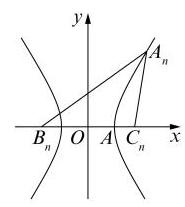
\includegraphics[width=0.2\textwidth]{bodyxb/src/49_634_1228_185_207_0.jpg}
        \end{center}

        \ps 设$a_n = a$，迭代可知$\left\{\begin{array}{l}
            b_{n+2} = b_n + \dfrac{a}{2} \\
            c_{n+2} = c_n + \dfrac{a}{2}
        \end{array}\right.$，故易知$\left\{  {S}_{{2n} - 1}\right\}$ 为严格增数列, $\left\{  {S}_{2n}\right\}$ 为严格增数列，结合选项可知选B.
    \end{jieda}

    \item (2024$\cdot$金山区一模$\cdot$12改)已知平面向量 $\vv{a}$ 、 $\vv{b}$ 、 $\vv{c}$ 满足 $\left| \vv{a}\right| = |\vv{c}| = 2$ ， $\left| {\vv{a} + \vv{b}}\right|  = \left| {\vv{a} - \vv{b}}\right|  + \left| \vv{a}\right|$ ，且 $\langle \vv{a},\vv{c}\rangle  = \dfrac{\pi }{3}$，若有$\vv{b} = \lambda \vv{a} + (1-\lambda)\vv{c}$，则 $\lambda = $\blkda[2]{$\dfrac{1}{4}$}.
    \begin{jieda}
        根据题意不妨设 $\vv{a} = \left( {2,0}\right)  = \vv{OA},\vv{b} = \left( {x,y}\right)  = \vv{OB}$ , $\vv{c} = \vv{OC},O$ 为坐标原点,则 $\left| {\vv{a} + \vv{b}}\right|  = \left| {\vv{a} - \vv{b}}\right|  + \left| \vv{a}\right|  \Longrightarrow  \sqrt{{\left( x + 2\right) }^{2} + {y}^{2}} = \sqrt{{\left( x - 2\right) }^{2} + {y}^{2}} + 2$ ,即点 $B$ 到 $\left( {-2,0}\right)$ 的距离比到点 $A$ 的距离大 2,根据双曲线的定义可知 $B$ 的轨迹为双曲线的一支,以 2 为长轴,4 为焦距,则 ${x}^{2} - \dfrac{{y}^{2}}{3} = 1(x >$ 1),又 $\langle \vv{a},\vv{c}\rangle  = \dfrac{\pi }{3}$ ,易知 $C$ 点轨迹为 $l : y =  \pm  \sqrt{3}x\left( {x > 0}\right)$ ,显然 $C$ 点轨迹为 $B$ 点轨迹双曲线的渐近线，又因为$|\vv{c}| = 2$，所以不妨设$C(1, \sqrt{3})$，根据$\vv{b} = \lambda \vv{a} + (1-\lambda)\vv{c}$可知$A, B, C$共线，联立求得$B\left(\dfrac{5}{4}, \dfrac{3\sqrt{3}}{4}\right)$，故$\lambda = \dfrac{1}{4}$.
    \end{jieda}

    \item (2025$\cdot$宝山区二模$\cdot$12)空间中有相互垂直的两条异面直线 ${l}_{1}$ 、 ${l}_{2}$ ，点 $A$ 、 $B \in  {l}_{1}$ ， $C$ 、 $D \in  {l}_{2}$ ，且 ${AB} =$ 4， ${CD} = 1$ ，若 ${DA}\bot {DB}$ ，且 ${AC} = {BC} + 2$ ，则二面角 $D - {AB} - C$ 平面角的余弦值最小为\blkda[2]{$\dfrac{4\sqrt{3}}{9}$}.
    \begin{jieda}
        根据双曲线的定义,平面内到两个定点 $A,B$ (焦点) 的距离之差的绝对值为定值 (小于 $\left| {AB}\right|$ ) 的点的轨迹为双曲线. 由 ${AC} = {BC} + 2$ ,可知点 $C$ 在以 $A,B$ 为焦点的双曲线靠近$B$的一支上. 在空间中,是此双曲线绕 ${AB}$ 旋转得到的曲面. 因为 ${DA} \bot  {DB}$ ,根据直径所对的圆周角是直角,所以点 $D$ 同时在以 ${AB}$ 为直径的球面上. 由于 ${l}_{1} \bot  {l}_{2}$ ,所以 $C,D$ 在与 ${AB}$ 垂直的面上. 
        
        设双曲线方程为 ${y}^{2} - \dfrac{{x}^{2}}{3} = 1$ . 过 $C$ 作 ${CE} \bot  {AB}$ 于 $E$，则$\angle CED$即为二面角 $D - {AB} - C$ 平面角.
        
        ${CE} =  \sqrt{3{y}^{2} - 3}$， ${DE} = \sqrt{4 - {y}^{2}}$ . 在 $\bigtriangleup  {CED}$ 中，根据余弦定理 $\cos \angle {CED}  = \dfrac{C{E}^{2} + D{E}^{2} - C{D}^{2}}{2 \cdot  {CE} \cdot  {DE}}$ ，通过 $C{E}^{2} = 3{y}^{2} - 3,D{E}^{2} = 4 - {y}^{2}$ 代入余弦定理公式化简得到, $\cos \angle {CED} = \dfrac{3{y}^{2} - 3 + 4 - {y}^{2} - 1}{2\sqrt{\left( {3{y}^{2} - 3}\right) \left( {4 - {y}^{2}}\right) }}  = \dfrac{\sqrt{3}}{3} \cdot  \sqrt{\dfrac{{y}^{4}}{-{y}^{4} + 5{y}^{2} - 4}} = \dfrac{\sqrt{3}}{3} \cdot  \sqrt{\dfrac{1}{-1 - \dfrac{4}{{y}^{4}} + \dfrac{5}{{y}^{2}}}}, y \in [-2, -1]$. 
        
        令 $t = \dfrac{1}{{y}^{2}}, t \in \left(\dfrac{1}{4}, 1\right)$ ,则 $\cos \angle {CED} = \dfrac{\sqrt{3}}{3} \cdot  \sqrt{\dfrac{1}{-4{t}^{2} + {5t} - 1}}$ . 对于二次函数 $f\left( t\right)  =  - 4{t}^{2} + {5t} - 1$ ,其对称轴为 $t =  - \dfrac{5}{2 \times  \left( {-4}\right) } = \dfrac{5}{8}$ , 当 $t = \dfrac{5}{8}$ 时, $f\left( t\right)$ 取得最大值 $f\left( \dfrac{5}{8}\right)  =  - 4 \times  {\left( \dfrac{5}{8}\right) }^{2} + 5 \times  \dfrac{5}{8} -  1 = \dfrac{9}{16}$ . 所以 $\cos \angle {CED} = \dfrac{\sqrt{3}}{3} \cdot  \sqrt{\dfrac{1}{-4{t}^{2} + {5t} - 1}} \geq  \dfrac{\sqrt{3}}{3}$ . $\sqrt{\dfrac{1}{\dfrac{9}{16}}} = \dfrac{4\sqrt{3}}{9}$.

        \begin{center}
        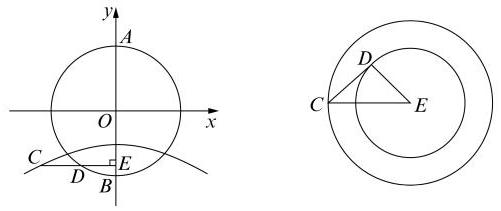
\includegraphics[width=0.4\textwidth]{bodyxb/src/120_285_568_501_211_0.jpg}
        \end{center}
    \end{jieda}
\end{enumerate}